
\chapter{基于双时相遥感影像特征交互的变化检测算法研究}
在变化检测任务中,基于深度学习的变化检测模型通常是在编码阶段,分别对双时相图像进行特征提取,然后基于双时相特征进行融合,以使得融合特征能够更好地表征变化信息。在本文中,将这种使用双时相影像特征融合或者交互表征变化特征的方法成为特征交互。在变化检测任务中,通常双时相特征交互的方法主要分为三种:一种是结合数学计算表现双时相特征图差异,比如结合向量距离计算~\cite{dong2024changeclip},差值计算~\cite{h_wei_spatio-temporal_2024}以及绝对值计算~\cite{shi_deeply_2022}等。第二种是基于注意力机制的特征交互方法,比如自注意力机制~\cite{Ying2024DGMA2NetAD}以及交叉注意力机制~\cite{lu_cross_2024}等。第三种是结合神经网络模块进行特征交互,比如特征拼接~\cite{chen2024changemamba}、特征交换~\cite{Fang2022ChangerFI}以及其他复杂的网络模块设计方法~\cite{Zhu2025Change3DRC}等。在本章中,重点针对第一种和第三种提出了本文的解决办法,分别从数学距离度量、特征交换以及复杂网络模块设计方法研究了表征变化特征的方法。

\section{基于特征层交换与欧氏距离差异特征计算的变化检测方法}
\subsection{引言}

遥感影像变化检测在环境监测、城市发展和水利领域中起着至关重要的作用。近年来,深度学习技术在遥感影像处理中的应用取得了显著进展。通过利用深度学习模型强大的特征拟合能力和高性能计算设备,遥感影像变化检测的准确性和效率得到了显著提升~\cite{Chen2021FCCDNFC}。这些深度学习模型能够处理大规模的遥感数据,识别和分析细微的地表变化,从而在环境监测中发挥越来越重要的作用。在遥感影像变化检测的深度学习领域,许多研究者从不同的研究层面优化了变化检测算法~\cite{chen_remote_2022, Fang2022ChangerFI}。变化检测算法的核心目标是检测双时相影像中发生变化的区域,模型需要识别在不同时间拍摄的两幅影像之间的变化区域。为了实现这一目标,可以关注两个主要方向:首先,增强模型从双时相影像中提取特征的能力,从而提高其对遥感影像的表示能力;其次,设计更精细的模块来表达差异特征,使变化检测模型更容易识别双时相影像中的变化区域。

具体而言,在特征提取骨干网络方面,一些研究者选择了先进的视觉变换器Vision Transformer~\cite{Dosovitskiy2020AnII}来提取双时相影像的特征。通过这些骨干网络强大的特征提取能力,模型在变化检测任务中的性能得到了提升~\cite{He2015DeepRL, Gu2023MambaLS, Dosovitskiy2020AnII}。与此同时,考虑到变化检测的独特性,许多研究者集中于差异特征的计算~\cite{dong_changeclip_2024, dong_efficientcd_2024}。因此,前述两类研究从不同的角度优化了变化检测任务。前者增强了模型对遥感影像中不同地物目标的理解,使得模型能够更好地识别双时相影像中的各种地物类别;后者则增强了模型对变化特征的感知能力,这是变化检测任务的基础。

\begin{figure}[!htbp]
  \centering
  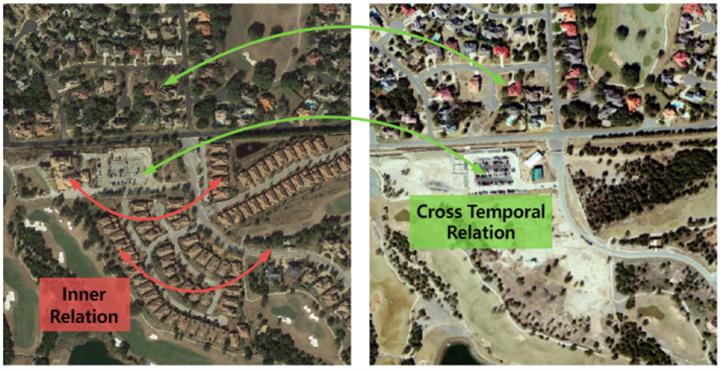
\includegraphics[width=\textwidth]{paper_figures/基于双时相遥感影像特征交互的变化检测算法研究/EfficientCD/efficientcd_relation.png}
  \caption{变化检测任务中的像素关系示意图}
  \label{fig:efficientcd_relation}
\end{figure}

在常见的变化检测算法中,通常使用拼接、加法和减法等方法来融合双时相特征,表示差异特征。从计算角度来看,特征拼接并不能直接反映双时相特征图之间的差异,它主要通过模型与变化标签之间的强拟合关系来学习变化区域~\cite{Daudt2018FullyCS}。加法保留了双时相影像中的前景区域,但模型需要学习哪些前景区域代表变化区域~\cite{gu2023fdff}。减法消除了双时相影像中相同元素的影响~\cite{feng_change_2023}。然而,减法方法增加了变化特征的数值差异,使得模型更难区分变化区域。因此,设计一种适合的方式来更好地构建差异特征的表示,一直是变化检测领域的研究热点。

在语义分割领域,特别是遥感影像分割中,不同层次特征的融合显著提高了模型的性能~\cite{Dong2021AMF, lin_feature_2017}。这些特征融合策略通过整合网络不同深度的信息,有效增强了模型识别图像中不同尺度和复杂度目标的能力。在遥感影像分割中,这种方法改善了对高空拍摄影像中细节变化的处理,如小尺度表面特征和复杂地形结构,从而实现了更精确的地物分类~\cite{wang2022unetformer}和变化检测~\cite{dong_changeclip_2024}。对于变化检测任务,独特的双时相影像为多层次特征融合提供了额外的优化方向~\cite{dong_changeclip_2024, Li2023MDFENetAM}。注意到,双时相影像中的地物类别存在显著相似性,如图~\ref{fig:efficientcd_relation}所示。因此,构建单时相影像内部以及双时相影像之间的像素依赖关系对增强模型的表示能力是有益的。

基于SEED架构中对变化检测任务中特征交换策略的阐述,本章提出了一种变化检测算法的优化方案,重点增强了单时相影像特征和双时相影像之间特征的交互。具体而言,本章的主要贡献如下:
\begin{itemize}
  \item 为了增强双时相遥感影像之间的特征交互,基于特征层交换的策略设计了ChangeFPN架构,通过无参数的方法改善双时相影像之间的特征传递。
  \item 基于特征图的欧几里得距离设计了一个逐层解码架构,用于变化检测任务。
\end{itemize}

\begin{figure}[!htbp]
  \centering
  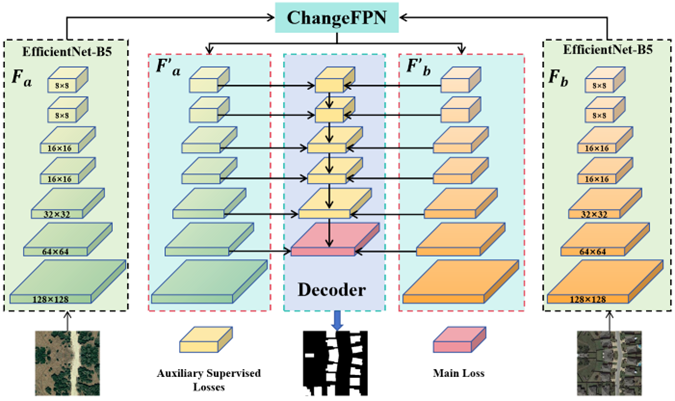
\includegraphics[width=\textwidth]{paper_figures/基于双时相遥感影像特征交互的变化检测算法研究/EfficientCD/efficientcd.png}
  \caption{EfficientCD的整体架构}
  \label{fig:efficientcd}
\end{figure}

\subsection{总体结构设计}

本章设计了一种基于EfficientNet骨干网络的变化检测网络,如图~\ref{fig:efficientcd}所示。该图展示了基于EfficientNet-B5骨干网络的变化检测模型。所提出的EfficientCD包括三部分:基于EfficientNet的特征提取骨干网络、用于促进不同层次双时相影像信息交换的ChangeFPN模块,以及逐层解码模块。骨干网络利用EfficientNet架构从输入影像中提取丰富且高效的特征,并且双编码器共享相同的权重。选择这一骨干网络是因为它在准确性和效率之间保持平衡,非常适合变化检测任务的需求,特别是在处理大型且复杂数据集时。ChangeFPN模块旨在增强从双时相影像中提取的不同层次特征之间的交互,如图~\ref{fig:efficientcd_changefpn}所示。通过允许对应层次的特征金字塔之间交换信息,ChangeFPN旨在提高模型检测和突出双时相影像之间变化的能力。最后,多层次解码模块从融合的金字塔特征图中逐步重建最终的变化检测图。这个逐层的方法确保了模型能够理解遥感影像中不同尺度的目标变化。在解码阶段,使用黄色特征图计算多个辅助损失,并使用红色特征图计算主损失。推理结果是从红色特征图中上采样得到的。

\begin{table}[!htbp]
\centering
\caption{EfficientNet-B5架构}
\label{tab:efficientnet-b5}
% 使用 booktabs 风格,移除竖线,并使用 c (居中) 和 l (左对齐)
\begin{tabular}{l l c c c c}
\toprule
\textbf{Stage} & \textbf{Operator} & \textbf{Kernel size} & \textbf{Resolution} & \textbf{Channels} & \textbf{Layers} \\
\midrule
1     & Conv       & $3\times3$     & $128\times128$  & 48       & 1      \\
2     & MBConv1    & $3\times3$     & $128\times128$  & 24       & 3      \\
3     & MBConv6    & $3\times3$     & $64\times64$    & 40       & 5      \\
4     & MBConv6    & $5\times5$     & $32\times32$    & 64       & 5      \\
5     & MBConv6    & $3\times3$     & $16\times16$    & 128      & 7      \\
6     & MBConv6    & $5\times5$     & $16\times16$    & 176      & 7      \\
7     & MBConv6    & $5\times5$     & $8\times8$      & 304      & 9      \\
8     & MBConv6    & $3\times3$     & $8\times8$      & 512      & 3      \\
\bottomrule
\end{tabular}
\end{table}


目前,大多数变化检测算法围绕视觉变换器(Vision Transformer,ViT)架构展开。视觉变换器架构中自注意力模块的全像素计算方法使得基于视觉变换器的特征提取骨干网络具备了遥感影像的全局认知能力。因此,利用视觉变换器架构的变化检测任务在多个数据集上取得了显著的成功。然而,通常由于自注意力模块中广泛的高维矩阵乘法计算,视觉变换器具有较高的计算成本。这种高计算需求也意味着模型在拟合遥感影像特征方面有更好的能力。

与上述方法不同,本章选择了轻量化网络结构EfficientNet作为变化检测任务的特征提取骨干网络。对于传统的卷积神经网络(CNNs),通过增加网络的深度和宽度来增强模型的拟合能力是可行的。然而,增加网络深度和宽度也会导致计算消耗的增加,并可能在网络训练过程中引发更严重的过拟合问题。变化检测任务通常以二分类为目标,专注于检测前景目标的变化区域。此外,与自然场景图像相比,遥感影像中包含的特定语义类别目标较少。因此,考虑到使用EfficientNet作为变化检测任务的特征提取骨干网络是合理的。为此,基于EfficientNet的结构特征,设计了图~\ref{fig:efficientcd}所示的特征提取骨干网络。选择EfficientNet-B5作为主要骨干网络,其架构结构见表\ref{tab:efficientnet-b5}。

表\ref{tab:efficientnet-b5}中提到的MBConv是架构中的一个模块,其中MBConv后面的数字(如1或6)表示扩展因子。这意味着MBConv模块中的第一个1x1卷积层会将输入特征矩阵的通道数扩展n倍。卷积核大小表示MBConv模块中深度可分离卷积~\cite{Chollet2016XceptionDL}使用的卷积核的大小。分辨率表示该阶段的输入分辨率。‘通道’指的是经过该阶段处理后输出特征矩阵中的通道数。‘层数’表示该阶段内操作结构的重复次数。

\begin{figure}[!htbp]
  \centering
  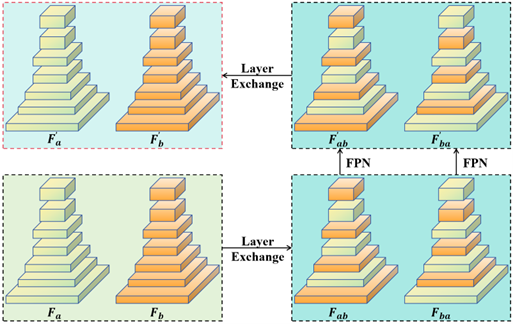
\includegraphics[width=\textwidth]{paper_figures/基于双时相遥感影像特征交互的变化检测算法研究/EfficientCD/efficientcd_changefpn.png}
  \caption{ChangeFPN中的特征交换方法示意图}
  \label{fig:efficientcd_changefpn}
\end{figure}

\subsection{结合特征层交换的变化检测FPN结构设计}

在计算机视觉领域,不同层次特征的融合增强了模型感知不同尺度目标的能力。然而,与语义分割任务不同,变化检测中的双时相影像地理位置保持不变,仅因时间变化导致影像中土地覆盖元素的差异。尽管如此,考虑到地理位置的一致性,双时相影像之间应该存在较强的相关性。为了使模型能够学习更多双时相影像之间的相关性,本章设计了ChangeFPN结构。如上图~\ref{fig:efficientcd_changefpn}所示,$F_{a}$ 和 $F_{b}$ 表示双时相影像的特征金字塔,${F}_{a}^{\prime}$ 和 ${F}_{b}^{\prime}$ 表示ChangeFPN的输出,与图~\ref{fig:efficientcd}相同。为了确保双时相影像之间信息的充分融合,本章选择了交换双时相特征金字塔相邻层的特征。 $F_{ab}$ 和 $F_{ba}$ 表示交换后的结果。同时对 $F_{ab}$ 和 $F_{ba}$ 应用了 FPN模型,生成了 ${F}_{ab}^{\prime}$ 和 ${F}_{ba}^{\prime}$。其中,$F_{ab}$ 和 $F_{ba}$ 具有彼此的特征层,通过FPN对 $F_{ab}$ 和 $F_{ba}$ 进行了多层次特征融合。最终得到的输出特征金字塔 ${F}_{ab}^{\prime}$ 和 ${F}_{ba}^{\prime}$ 融合了双时相影像的特征。通过这种计算方法,不仅加强了不同层次的信息融合,还构建了双时相影像特征图之间的信息融合。为了确保特征交换方法不会影响后续解码部分,使用了层交换计算进行恢复。与其他基于特征的方法不同,这些方法构建了双时相影像特征之间的交互,基于层次的方法巧妙地增加了双时相影像之间的信息交换,从而提高了变化检测模型感知变化特征的能力,同时没有增加计算负担。

\subsection{结合欧氏距离差异特征计算的变化检测解码器}

在EfficientCD的解码阶段,本章采用了分层的方法处理ChangeFPN输出的特征,并计算了每个层次上双时相特征图之间的变化,如图\ref{fig:efficientcd_euclidean}所示。对于FPN模块中的每一层双时相特征图,首先沿着通道维度C将双时相特征图(标记为F1和F2)拼接,形成一个合并的特征图。随后,计算这两个特征图之间的欧几里得距离,以估算双时相特征图之间的差异程度。计算欧几里得距离的公式如下:
\begin{align}
D &= \sqrt{\sum_{c}(F_{1} - F_{2})^{2}} \label{func:efficientcd-1} \\
D_{\mathrm{norm}} &= \sigma\!\Bigl(\frac{D}{D_{\max}}\Bigr) \label{func:efficientcd-2}
\end{align}


在公式(1-3)中, D表示F1和F2之间的欧几里得距离矩阵, $\sigma$表示sigmoid函数,${D_{\max}}$为欧几里得距离的最大值,$D_{\mathrm{norm}}$是归一化后的距离。在图\ref{fig:efficientcd_euclidean}中,左侧的紫色模块表示双时相特征图F1和F2。首先,双时相特征图F1和F2被拼接生成一个融合的特征图。然后,融合特征图经过一个残差块处理,同时添加来自前一层的解码特征图,构建了解码阶段的逐层特征融合。融合特征图接着经过双线性插值上采样,以恢复其空间分辨率。上采样后的特征图进一步经过另一个残差块处理。为了增强模型对变化区域的敏感性,双时相特征图F1和F2通过欧几里得距离模块计算差异图,如公式\ref{func:efficientcd-1}和\ref{func:efficientcd-2}所示。差异图也经过双线性插值上采样,以匹配特征图的分辨率。然后,上采样后的差异图和特征图逐元素相乘,增强了变化显著区域的特征。这些步骤构成了一个结合欧几里得距离的解码模块,有效提高了模型在逐层解码和特征融合中检测变化的能力。逐层解码方法更适合遥感影像密集预测任务,因为遥感图像识别通常需要结合不同层次的特征信息,以获得更好的识别效果。

\begin{figure}[!htbp]
  \centering
  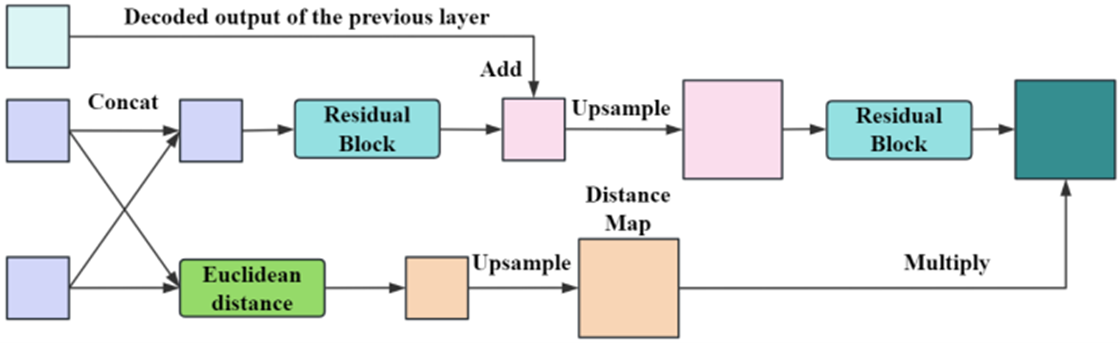
\includegraphics[width=\textwidth]{paper_figures/基于双时相遥感影像特征交互的变化检测算法研究/EfficientCD/efficientcd_euclidean.png}
  \caption{结合欧几里得距离计算的双时相差异特征融合模块示意图。}
  \label{fig:efficientcd_euclidean}
\end{figure}

\begin{figure}[!htbp]
  \centering
  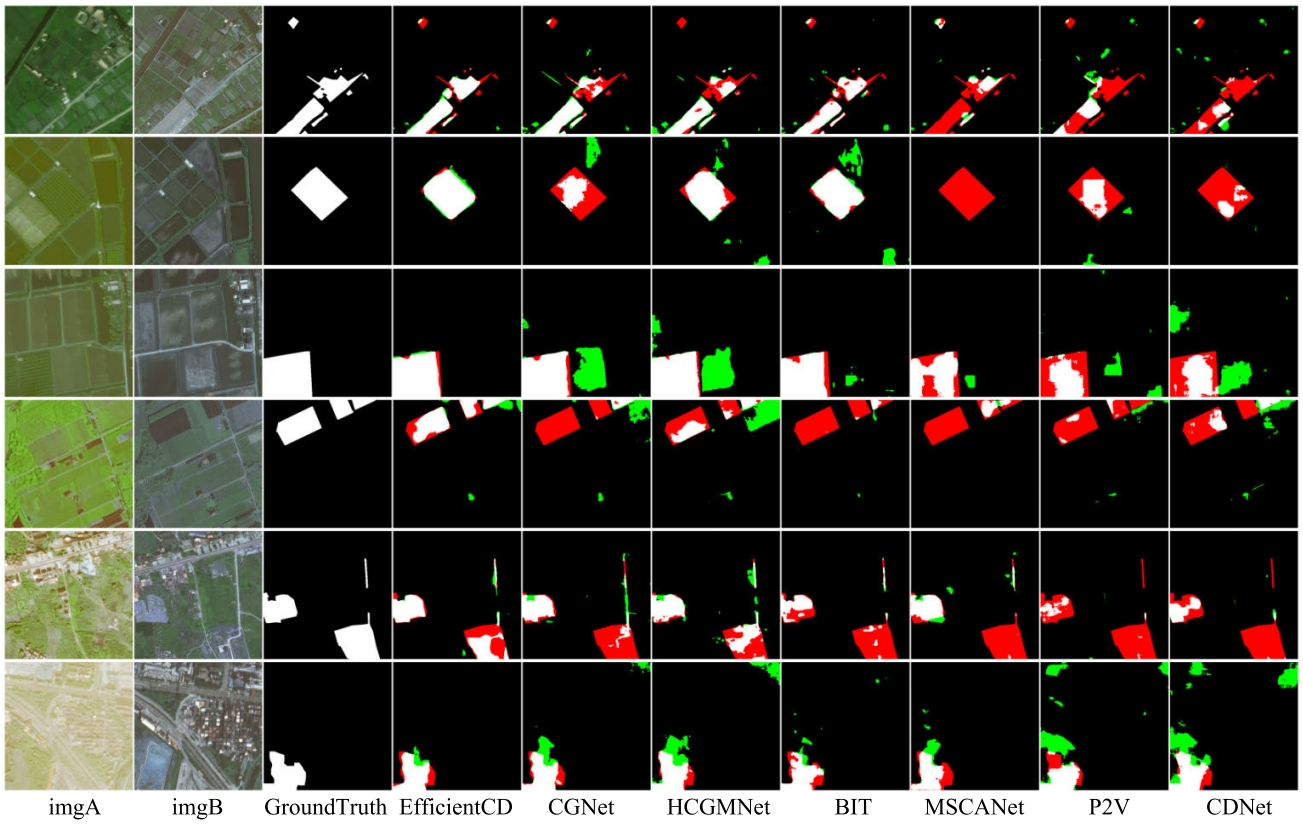
\includegraphics[width=\textwidth]{paper_figures/基于双时相遥感影像特征交互的变化检测算法研究/EfficientCD/efficientcd_clcd.png}
  \caption{EfficientCD 模型与对比模型在CLCD数据集上的可视化对比结果}
  \label{fig:efficientcd_clcd}
\end{figure}

\begin{figure}[!htbp]
  \centering
  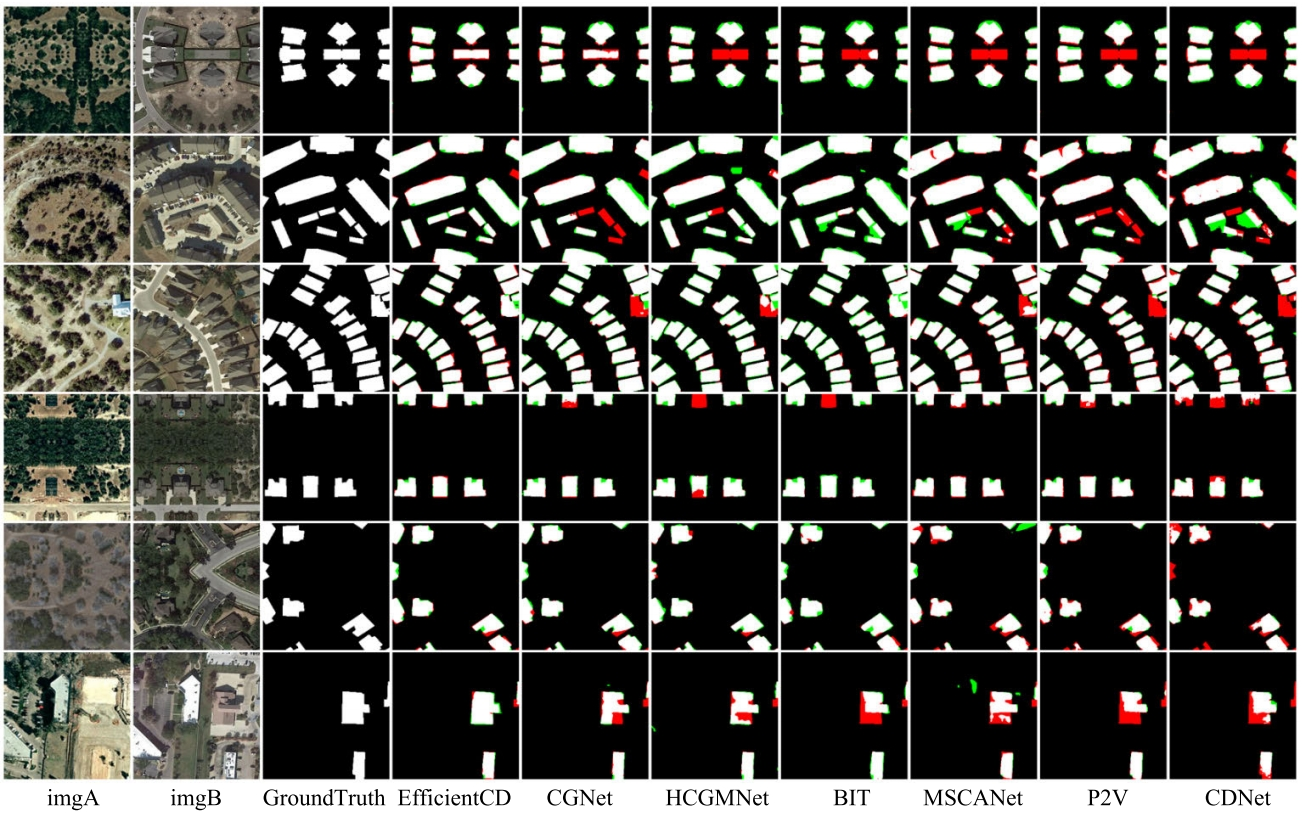
\includegraphics[width=\textwidth]{paper_figures/基于双时相遥感影像特征交互的变化检测算法研究/EfficientCD/efficientcd_levir.png}
  \caption{fficientCD 模型与对比模型在 LEVIR-CD 数据集上的可视化对比结果}
  \label{fig:efficientcd_levir}
\end{figure}

\subsection{实验结果与分析}


\begin{figure}[!htbp]
  \centering
  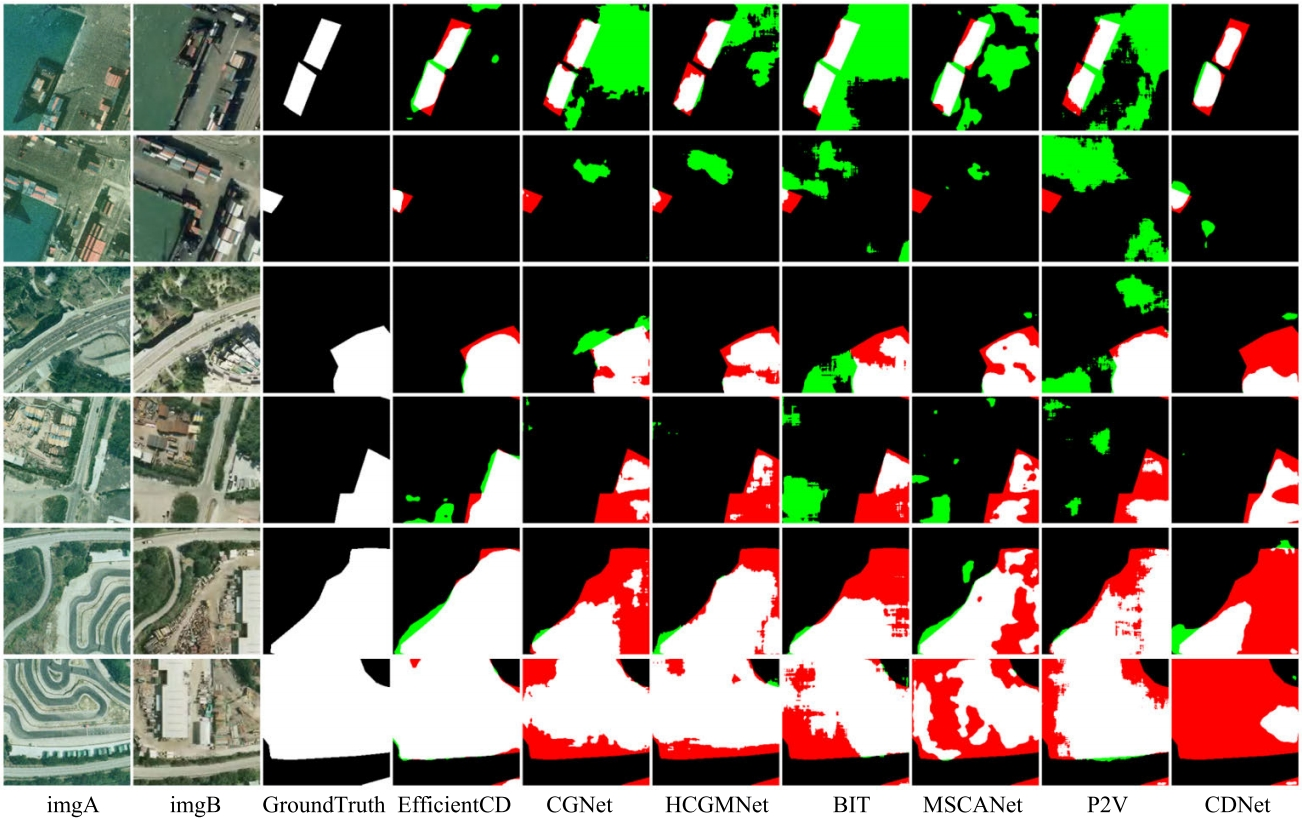
\includegraphics[width=\textwidth]{paper_figures/基于双时相遥感影像特征交互的变化检测算法研究/EfficientCD/efficientcd_sysu.png}
  \caption{EfficientCD 模型与对比模型在 SYSU-CD 数据集上的可视化对比结果}
  \label{fig:efficientcd_sysu}
\end{figure}


\subsubsection{实验结果量化指标与可视化分析}

如表~\ref{tab:efficientcd_clcd}、表~\ref{tab:efficientcd_levir}、表~\ref{tab:efficientcd_whucd}和表~\ref{tab:efficientcd_sysu},在四个数据集上对EfficientCD进行了广泛的评估:CLCD、LEVIR-CD、WHUCD和SYSU-CD。根据主要评估指标,EfficientCD在所有数据集上均取得了最先进的性能。符号``--''表示原始论文中缺失的数据。对于这些情况,重新训练了部分模型以提高准确性。由于这些是二分类变化检测任务,前景变化类别的交并比(IoU)作为主要指标。对四个数据集性能的详细比较明确展示了EfficientCD算法在关键评估指标上的优越性。特别是在IoU指标方面,EfficientCD不仅在每个数据集上都取得了最高得分,而且还表现出了显著的优势:在CLCD数据集上,EfficientCD的IoU为65.14\%,超过第二名CGNet(62.67\%)约2.47个百分点;在LEVIR-CD数据集上,其IoU为85.55\%,略高于CGNet(85.40\%)0.15个百分点;在SYSU-CD数据集上,EfficientCD的IoU飙升至71.53\%,超过第二名SSANet(68.18\%)3.35个百分点;在WHUCD数据集上,EfficientCD的IoU为90.71\%,超越CGNet(90.41\%)0.3个百分点。这些比较数据突显了EfficientCD在精确识别遥感影像中的变化区域方面的高效性和准确性,充分证明了其在遥感影像变化检测领域的先进地位和优越性。

\begin{figure}[!htbp]
  \centering
  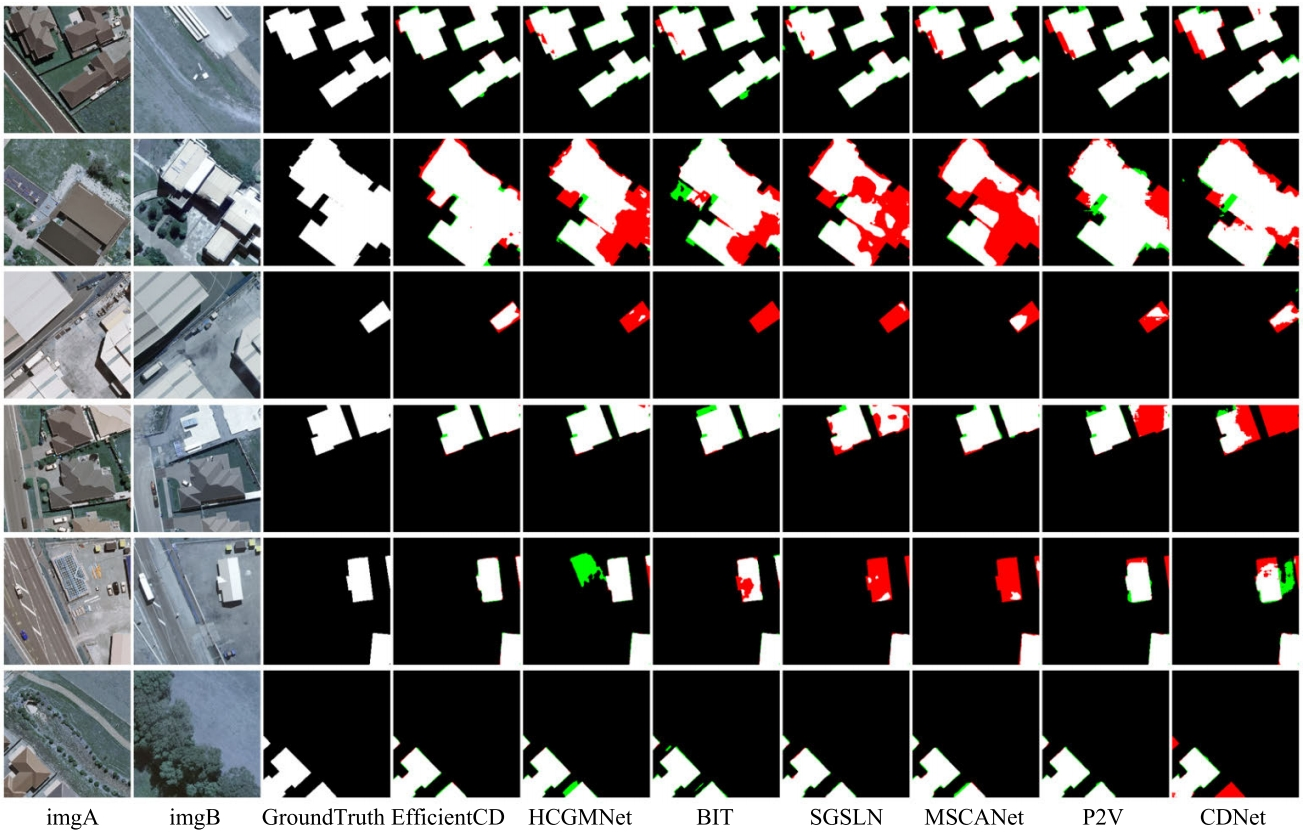
\includegraphics[width=\textwidth]{paper_figures/基于双时相遥感影像特征交互的变化检测算法研究/EfficientCD/efficientcd_whucd.png}
  \caption{EfficientCD 模型与对比模型在 WHUCD 数据集上的可视化对比结果}
  \label{fig:efficientcd_whucd}
\end{figure}

在图~\ref{fig:efficientcd_clcd}、图~\ref{fig:efficientcd_levir}、图~\ref{fig:efficientcd_sysu}和图~\ref{fig:efficientcd_whucd}中,提供了CLCD、LEVIR-CD、SYSU-CD和WHUCD的测试结果可视化。选择了EfficientCD在IoU指标上得分最高的模型,并与近年来的经典算法进行了比较。在这些可视化结果中,真正阳性(TP)用白色像素表示,真正阴性(TN)用黑色像素表示,假阳性(FP)用绿色像素表示,假阴性(FN)用红色像素表示。可视化结果明确表明,EfficientCD在多样化数据集和应用场景中均展现出卓越的检测性能,与真实标注结果高度吻合。

\begin{table}[!htbp]
  \centering
  \caption{EfficientCD 模型与经典变化检测模型在 CLCD 数据集上的定量对比结果}
  \label{tab:efficientcd_clcd}
  \begin{tabular}{lccccc}
    \toprule
    Model              &  OA   &  IoU  &  F1   &  Rec  & Prec  \\
    \midrule
    CDNet~\cite{Alcantarilla2016StreetviewCD}              & 95.27 & 48.31 & 65.15 & 59.43 & 72.09 \\
    P2V~\cite{lin_transition_2023}                & 95.84 & 54.10 & 70.22 & 65.93 & 75.11 \\
    MSCANet~\cite{m_liu_cnn-transformer_2022}            & 96.05 & 55.83 & 71.65 & 67.07 & 76.91 \\
    BIT~\cite{chen_remote_2022}                & 96.46 & 58.36 & 73.71 & 66.63 & 82.47 \\
    DSIFN~\cite{Zhang2020ADS}              & 96.55 & 59.42 & 74.54 & 67.86 & 82.69 \\
    HCGMNet~\cite{Han2023HCGMNetAH}            & 96.27 & 59.58 & 74.67 & 73.92 & 75.44 \\
    GaMPF~\cite{Zhao2024GaMPFAF}              & 96.68 & 60.52 & 75.40 & 68.36 & 84.06 \\
    AMTNet~\cite{Liu2023AnAM}             &  --   & 62.35 & 76.81 & 75.06 & 78.64 \\
    CGNet~\cite{han_change_2023}              & 96.82 & 62.67 & 77.05 & 71.71 & 83.25 \\
    EfficientCD (B5)   & 96.98 & 65.14 & 78.89 & 75.83 & 82.21 \\
    \bottomrule
  \end{tabular}
\end{table}


\begin{table}[!htbp]
  \centering
  \caption{EfficientCD 模型与经典变化检测模型在 LEVIR-CD 数据集上的定量对比结果}
  \label{tab:efficientcd_levir}
  \begin{tabular}{lccccc}
    \toprule
    Model            &   OA   &  IoU   &   F1   &  Rec   &  Prec   \\
    \midrule
    CDNet~\cite{Alcantarilla2016StreetviewCD}            &  98.35 &  72.21 &  83.87 &  84.14 &  83.61  \\
    BIT~\cite{chen_remote_2022}              &  98.95 &  80.86 &  89.48 &  87.53 &  90.65  \\
    MSCANet~\cite{m_liu_cnn-transformer_2022}          &  99.03 &  81.91 &  90.06 &  86.38 &  94.06  \\
    MFATNet~\cite{Mao2022MFATNetMF}          &  99.03 &  82.42 &  90.36 &  88.93 &  91.85  \\
    ChangeFormer~\cite{bandara2022transformer}     &  99.04 &  82.66 &  90.50 &  90.18 &  90.83  \\
    P2V~\cite{lin_transition_2023}              &  99.04 &  83.00 &  90.71 &  91.78 &  89.67  \\
    AMTNet~\cite{Liu2023AnAM}           &   --   &  83.08 &  90.76 &  89.71 &  91.82  \\
    DMATNet~\cite{Song2022RemoteSI}          &  98.25 &  84.13 &  90.75 &  89.98 &  91.56  \\
    STransUNet~\cite{Yuan2022STransUNetAS}       &  99.13 &  84.19 &  91.41 &  90.55 &  92.30  \\
    HCGMNet~\cite{Han2023HCGMNetAH}          &  99.18 &  85.26 &  92.04 &  92.81 &  91.29  \\
    Changer~\cite{Fang2022ChangerFI}        &   --   &  85.29 &  92.06 &  90.56 &  93.61  \\
    CGNet~\cite{han_change_2023}            &  99.20 &  85.40 &  92.13 &  91.93 &  92.32  \\
    EfficientCD (B5) &  99.22 &  85.55 &  92.21 &  91.22 &  93.23  \\
    \bottomrule
  \end{tabular}
\end{table}



\begin{table}[!htbp]
  \centering
  \caption{EfficientCD 模型与经典变化检测模型在 SYSU-CD 数据集上的定量对比结果}
  \label{tab:efficientcd_sysu}
  \begin{tabular}{lccccc}
    \toprule
    Model          &   OA   &  IoU   &   F1   &   Rec   &  Prec   \\
    \midrule
    MSCANet~\cite{m_liu_cnn-transformer_2022}        &  89.99 &  63.04 &  77.33 &  72.40  &  82.99  \\
    CDNet~\cite{Alcantarilla2016StreetviewCD}          &  89.90 &  64.34 &  78.30 &  77.29  &  79.34  \\
    DSAMNet~\cite{shi_deeply_2022}        &   --   &  64.18 &  78.18 &  81.86  &  74.81  \\
    ISNet~\cite{Cheng2022ISNetTI}          &  90.01 &  64.44 &  78.29 &  80.27  &  76.41  \\
    BIT~\cite{chen_remote_2022}            &  90.57 &  64.81 &  78.65 &  73.68  &  84.34  \\
    SNUNet~\cite{Fang2021SNUNetCDAD}         &  90.79 &  66.02 &  79.54 &  75.87  &  83.58  \\
    L-UNet~\cite{Papadomanolaki2021ADM}         &  90.58 &  66.15 &  79.63 &  78.08  &  81.24  \\
    P2V~\cite{lin_transition_2023}            &  90.49 &  66.29 &  79.73 &  79.29  &  80.17  \\
    HCGMNet~\cite{Han2023HCGMNetAH}        &  91.12 &  66.33 &  79.76 &  74.15  &  86.28  \\
    CGNet~\cite{han_change_2023}          &  91.19 &  66.55 &  79.92 &  74.37  &  86.37  \\
    DARNet~\cite{li_densely_2022}         &  91.26 &  68.10 &  81.03 &  79.11  &  83.04  \\
    SSANet~\cite{Jiang2022JointVL}         &   --   &  68.18 &  81.08 &  79.73  &  82.48  \\
    SGSLN~\cite{zhao_exchanging_2023}          &   --   &  71.05 &  83.07 &  81.45  &  84.76  \\
    EfficientCD (B5)& 92.46 &  71.53 &  83.40 &  80.27  &  86.78  \\
    \bottomrule
  \end{tabular}
\end{table}


\begin{table}[!htbp]
  \centering
  \caption{EfficientCD 模型与经典变化检测模型在 WHUCD 数据集上的定量对比结果}
  \label{tab:efficientcd_whucd}
  \begin{tabular}{lccccc}
    \toprule
    Model            &   OA   &  IoU   &   F1   &   Rec   &  Prec   \\
    \midrule
    CDNet~\cite{Alcantarilla2016StreetviewCD}            &  98.96 &  79.59 &  88.63 &  87.24  &  90.07  \\
    SNUNet~\cite{Fang2021SNUNetCDAD}           &  99.24 &  84.69 &  91.71 &  90.77  &  92.67  \\
    P2V~\cite{lin_transition_2023}              &  99.31 &  85.91 &  92.42 &  90.93  &  93.97  \\
    DSIFN~\cite{Zhang2020ADS}            &  99.34 &  86.36 &  92.68 &  90.20  &  95.30  \\
    MSCANet~\cite{m_liu_cnn-transformer_2022}          &  99.36 &  86.65 &  92.85 &  89.98  &  95.90  \\
    SGSLN~\cite{zhao_exchanging_2023}            &  99.38 &  87.47 &  93.32 &  92.91  &  93.72  \\
    BIT~\cite{chen_remote_2022}              &  99.43 &  88.22 &  93.74 &  92.00  &  95.56  \\
    HCGMNet~\cite{Han2023HCGMNetAH}          &  99.52 &  90.10 &  94.79 &  95.31  &  94.27  \\
    CGNet~\cite{han_change_2023}            &  99.54 &  90.41 &  94.96 &  94.61  &  95.32  \\
    EfficientCD (B5) &  99.55 &  90.71 &  95.13 &  94.19  &  96.08  \\
    \bottomrule
  \end{tabular}
\end{table}

\begin{table}[!htbp]
  \centering
  \setlength{\tabcolsep}{3pt} % 调整列间距
  \caption{基于IoU指标的EfficientCD 模型消融实验}
  \label{tab:efficientcd_ablation}
  \begin{tabular}{lcccccc}
    \toprule
    Model         & ChangeFPN & Decoder & LEVIR-CD & SYSU-CD & CLCD   & WHUCD  \\
    \midrule
    EfficientCD   & ×         & ×       & 84.32    & 64.43   & 61.41  & 88.27  \\
                  & √         & ×       & 84.96    & 68.40   & 62.82  & 90.32  \\
                  & ×         & √       & 85.31    & 66.94   & 62.38  & 89.20  \\
                  & √         & √       & 85.55    & 71.53   & 65.14  & 90.71  \\
    \bottomrule
  \end{tabular}
\end{table}

\begin{table}[!htbp]
  \centering
  \setlength{\tabcolsep}{3pt}
  \caption{基于IoU指标的针对不同骨干网络的EfficientCD模型消融实验}
  \label{tab:efficientcd_backbone}
  \begin{tabular}{lcccccc}
    \toprule
    Backbone         & Params (M) & FLOPs (G) & LEVIR-CD & SYSU-CD & WHUCD & CLCD   \\
    \midrule
    EfficientNet-B0  &   48.21    &   45.24   &  84.69   &  68.92  & 90.22 & 65.30  \\
    EfficientNet-B1  &   50.71    &   45.74   &  84.82   &  69.58  & 90.06 & 61.52  \\
    EfficientNet-B2  &   52.05    &   45.96   &  84.74   &  68.56  & 90.04 & 63.09  \\
    EfficientNet-B3  &   55.19    &   46.77   &  84.54   &  68.02  & 90.17 & 62.38  \\
    EfficientNet-B4  &   62.34    &   48.18   &  84.34   &  67.58  & 89.71 & 62.38  \\
    EfficientNet-B5  &   73.43    &   50.42   &  85.55   &  71.53  & 90.71 & 64.61  \\
    ResNet18         &   48.84    &   48.30   &  83.80   &  64.65  & 80.88 & 50.91  \\
    ResNet34         &   58.95    &   53.12   &  82.69   &  64.97  & 82.13 & 50.94  \\
    ResNet50         &   61.91    &   54.66   &  83.35   &  65.85  & 82.83 & 49.44  \\
    ResNeSt14d       &   46.96    &   51.14   &  83.80   &  66.47  & 86.31 & 55.57  \\
    ResNeSt26d       &   53.42    &   53.44   &  81.39   &  66.70  & 81.05 & 53.78  \\
    ResNeSt50d       &   63.84    &   58.03   &  73.17   &  62.74  & 72.30 & 50.65  \\
    Swin-Tiny        &   62.63    &   42.41   &  85.27   &  68.12  & 90.13 & 63.59  \\
    Swin-Small       &   83.95    &   50.93   &  85.64   &  68.28  & 90.85 & 64.65  \\
    Swin-Base        &  122.00    &   64.37   &  85.62   &  68.38  & 88.91 & 63.19  \\
    ConvNeXt-Nano    &   50.00    &   49.99   &  84.85   &  66.14  & 88.91 & 58.14  \\
    ConvNeXt-Small   &   62.93    &   55.29   &  84.69   &  65.25  & 89.08 & 59.21  \\
    ConvNeXt-Tiny    &   84.57    &   66.35   &  84.92   &  64.84  & 88.76 & 58.32  \\
    \bottomrule
  \end{tabular}
\end{table}



\subsubsection{消融实验}

消融研究聚焦于四个数据集(LEVIR-CD、SYSU-CD、CLCD和WHUCD)上的交并比(IoU)指标,揭示了将ChangeFPN和解码器引入EfficientCD算法的显著影响。在表~\ref{tab:efficientcd_ablation}中,在基线模型中没有使用ChangeFPN和结合欧几里得距离的逐层解码器。首先,基于EfficientNet-B5骨干网络构建了一个特征图金字塔,然后通过拼接融合特征图金字塔,并使用FPN处理双时相影像的融合特征。最后,将处理后的特征图通过逐层上采样融合恢复成预测结果。在ChangeFPN的消融实验中,去除了在EfficientCD完整网络中交换双时相影像层次特征的步骤。在解码器的消融实验中,将EfficientCD的解码器部分修改为与基线模型一致。消融结果不仅展示了ChangeFPN和解码器对算法准确性提升的独立贡献,还表明它们之间存在协同效应,推动EfficientCD算法达到了最佳的性能水平。这项消融研究明确说明了ChangeFPN和解码器在提高遥感影像变化检测精度中的关键作用,强调了它们对EfficientCD算法整体效果的不可或缺的贡献。

\subsection{讨论}

\subsubsection{EfficientNet在变化检测中的应用}

本章采用EfficientNet骨干网络作为变化检测算法的特征提取模块。在二分类变化检测任务中,特征提取部分通常需要考虑两个方面。一方面,可以通过增强骨干算法的特征提取能力来优化变化检测算法,例如BIT~\cite{chen_remote_2022}、SwinSUNet~\cite{Zhang2022SwinSUNetPT}等。另一方面,考虑到模型在二分类变化检测任务中主要关注变化区域,使用了一个更轻量化的模型来进行特征提取。这种方法不仅减少了模型的参数数量,从而加快了推理速度,而且还保证了特征提取骨干网络的轻量化有助于防止过拟合。

此外,为了测试不同深度的EfficientNet模型在不同变化检测数据集上的表现,对从B0到B5的EfficientNet模型进行了测试,测试结果如表~\ref{tab:efficientcd_backbone}所示。由于缺少预训练模型,EfficientNet-B6和EfficientNet-B7未包含在对比实验中。从结果来看,基于EfficientNet骨干的模型在变化检测任务中可以取得较好的效果。此外,模型在不同数据集上的准确度并未与EfficientNet模型的深度呈现正相关。

作为EfficientCD算法的骨干,EfficientNet-B5在多个数据集上表现出色,尤其是在SYSU-CD和LEVIR-CD数据集上,凭借其优越的IoU得分,表明其在复杂的遥感影像变化检测任务中具有很高的有效性。尽管其相对较高的参数数量和计算复杂度,EfficientNet-B5与其他高性能模型如Swin Transformer~\cite{Liu2021SwinTH}和ConvNeXt~\cite{Liu2022ACF}系列相比,在效率和精度之间仍然保持了很好的平衡。这个平衡展示了EfficientNet-B5优化网络设计的优势,虽然参数稍有增加,但在多个数据集上达到了更高的准确度。该模型能够在合理的计算需求下保持高精度,使EfficientNet-B5成为高精度遥感变化检测的理想选择,确保通过在精度和计算效率之间实现最佳平衡,EfficientCD在各种数据集上都能表现出色。

\subsubsection{变化检测中的特征交换}

如上述实验部分所示,在双时相特征金字塔中交换了特征图以进行变化检测任务。在不增加参数数量的情况下,ChangeFPN促进了变化检测任务的实现。参考现有的研究~\cite{Fang2022ChangerFI},在变化检测任务中对双时相特征图进行空间或通道交换,可以优化模型的检测结果并增强其泛化能力。在深度学习模型的特征金字塔中,来自原始图像的不同层次特征被提取出来。不同层次特征图之间的信息交换帮助模型更好地理解图像特征,学习图像中不同尺度的目标。因此,本章在双时相特征图上进行了特征交换。一方面,对于双时相影像,ChangeFPN促进了来自不同时间的影像特征之间的信息交互,增强了变化检测模型的表示能力。另一方面,对于单时相影像,模型通过引入来自另一个时间阶段的特征图,从而为单时相特征提取组件补充了额外的信息。

\subsection{小结}

本章基于EfficientNet的结构特征设计了一个多层次特征金字塔,用于提取双时相特征。同时,在不增加额外参数的情况下,设计了适合变化检测任务的ChangeFPN模块,基于FPN结构有效增强了双时相影像特征之间的信息交换。最后,在解码器部分,结合了欧几里得距离计算,设计了一个逐层解码器,直观地展示了双时相特征图之间的差异。实验结果表明,EfficientCD在多个标准数据集上表现优异,展示了其在处理复杂场景和大规模数据时的高效性。此外,提出的ChangeFPN展示了很高的灵活性和可扩展性,可以灵活地添加到基于Bi-Encoder-Neck-Decoder架构的变化检测算法中。总之,EfficientCD有效地促进了变化检测任务的效果,为未来变化检测算法的研究提供了有益的启示。


\section{基于特征层交换的与通道-空间差异计算的变化检测方法}
\subsection{引言}

深度学习技术的兴起为遥感变化检测带来了新的契机,并取得了显著进展~\cite{ting_bai_deep_2023}。卷积神经网络(CNN)~\cite{He2015DeepRL}和 Transformer~\cite{Vaswani2017AttentionIA}等深度模型凭借其强大的特征提取与模式识别能力,能够从海量数据中自动学习到高效的表征,大幅提升变化检测的准确性与效率。随着计算资源的提升和大规模遥感数据集的不断积累,将深度学习融入地球观测已成为研究热点~\cite{Wang2024HyperSIGMAHI}。这一范式不仅推动了变化检测性能的提升,也加速了智能地球观测系统的发展,为更高鲁棒性和可扩展性的解决方案奠定了基础。

在基于深度学习的模式识别任务中,特征提取是成功的关键。研究者不断改进特征提取网络,以推动下游任务的发展~\cite{He2015DeepRL, Dosovitskiy2020AnII, Liu2021SwinTH}。在语义分割任务中,模型通过识别单张输入图像中的目标和区域进行学习;为提升分割性能,常见策略包括扩展感受野和融合上下文信息,使模型能够更好地捕捉和表征图像特征~\cite{chen2018encoder, Wang2024PyramidMambaRP}。

\begin{figure}[!htbp]
  \centering
  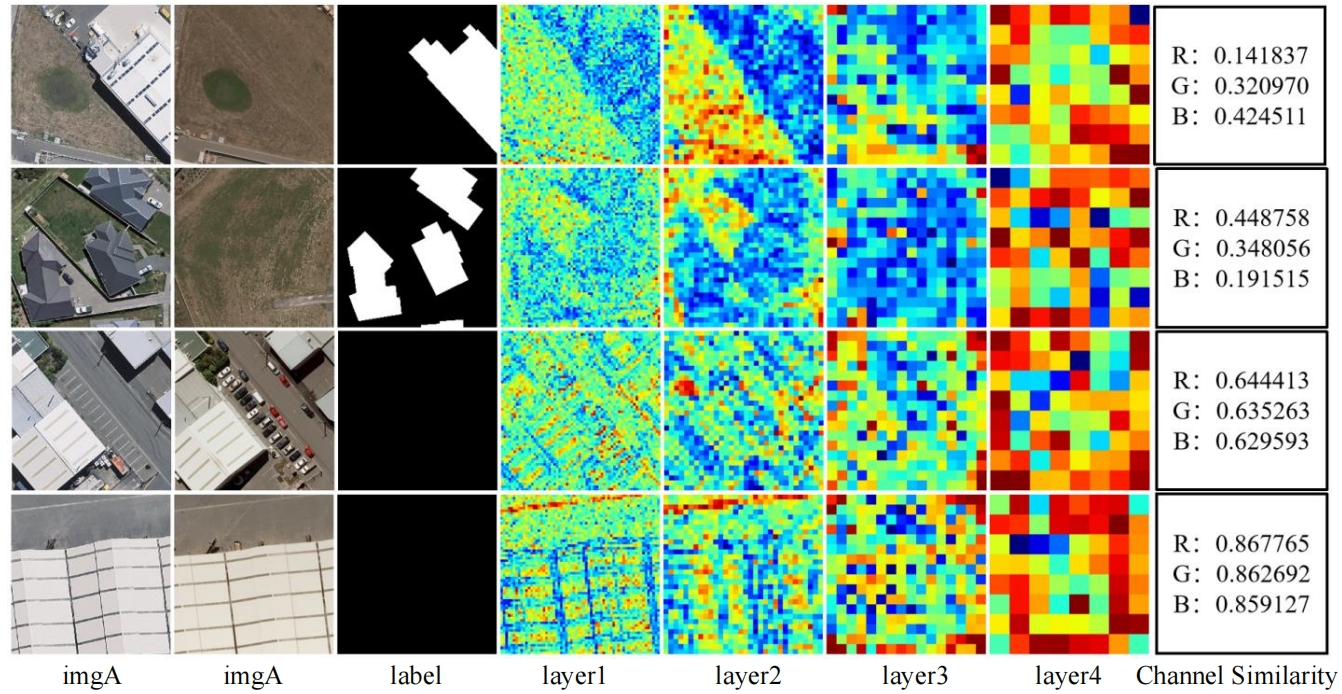
\includegraphics[width=\textwidth]{paper_figures/基于双时相遥感影像特征交互的变化检测算法研究/LENet/lenet_similarity.png}
  \caption{变化检测影像在不同维度下差异的表现形式。Layer1 至 Layer4 的计算方法:采用 Swin Transformer V2 对图像进行编码,并分别计算空间维度上的余弦相似度。Channel Similarity 的计算方法:将双时相图像按 RGB 通道展平成向量,计算两向量之间的余弦相似度。}
  \label{fig:lenet_similarity}
\end{figure}

变化检测同样是一种像素级识别任务,但与单图输入的语义分割不同,它需要将双时相图像同时输入网络,以识别随时间发生变化的区域。因此,研究者们指出,变化检测不仅需要对单张图像具备强大的特征拟合能力,还需构建双时相特征之间的交互机制,以增强模型对变化信息的学习能力~\cite{dong_changeclip_2024, Noman2023RemoteSC, zhao_exchanging_2023},从而提升整体检测性能。

针对特征交互机制,已有多种方案问世。一些工作基于注意力机制构建时空交互~\cite{Peng2024FDAFFNetAF, Dong2024ISANetAI},也有研究采用传统卷积模块实现交互~\cite{b_huang_remote-sensing_2024, Zhang2020ADS}。在 Changer 模型中,Fang 等人~\cite{Fang2022ChangerFI}系统地分析了聚合-分布、通道交换、空间交换和基于流的双向对齐融合等多种交互方案,凸显出为变化检测任务量身设计复杂交互机制的重要性。

与以往研究不同,本章提出了一种新颖的差异特征学习机制,以构建双时相特征之间的交互。如图~\ref{fig:lenet_similarity}所示,在变化检测任务中采用余弦相似度来计算双时相图像的空间和通道相似度。其中,“layer1–layer4”表示在空间维度上计算得到的相似度矩阵(热力图)。从这些热力图中可以看到,变化区域在空间特征图上的相似度值相对较低,而未变化区域的相似度值相对较高。对于通道相似度,分别取原始双时相图像的每个 RGB 波段,将每个单波段图像展平成一维向量,然后计算相应向量之间的余弦相似度。得到的通道相似度值表明,变化区域在所有三个 RGB 通道上的相似度均较低,而未变化区域在各通道上的相似度均较高。这些观察结果表明,在双时相图像的空间和通道维度上计算变化特异性差异是可行的。

通常,传统差异特征学习多聚焦于空间差异~\cite{dong_changeclip_2024, feng_change_2023, shi_deeply_2022}。相较而言,本章的方法引入了基于通道的全局差异计算,能够捕捉更全面、细粒度的变化信息。通过将空间差异信息与通道差异信息相结合,设计了一个基于余弦相似度算法的通道-空间差异加权(Channel-Space Differential Weighting,CSDW)模块。该模块使双时相特征图能够更有效地聚焦于变化区域,从而提升变化检测的准确性和鲁棒性。基于SEED架构的思想,解码阶段采用了以特征层交换策略为基础的逐层交换解码器(Layer-Exchange Decoder, LED),通过层与层之间的交换机制,逐步增强特征交互。该设计使模型能够更好地利用双时相图像之间的时序依赖,从而获得更精确、可靠的变化检测结果。本章的主要贡献总结如下:

\begin{itemize}
  \item 针对变化检测任务,设计了一种新颖的差异特征学习模块,通过计算双时相特征在空间和通道维度的信息差异,既捕捉局部变化,也获取全局变化信息,有效弥补了传统仅基于空间方法的局限性。
  \item 提出了逐层交换解码器(LED),通过层与层之间的特征交换机制,逐步增强双时相特征的交互,提升模型对时序依赖和空间关联的捕捉能力,从而实现更高精度的变化检测。
\end{itemize}


\begin{figure}[!htbp]
  \centering
  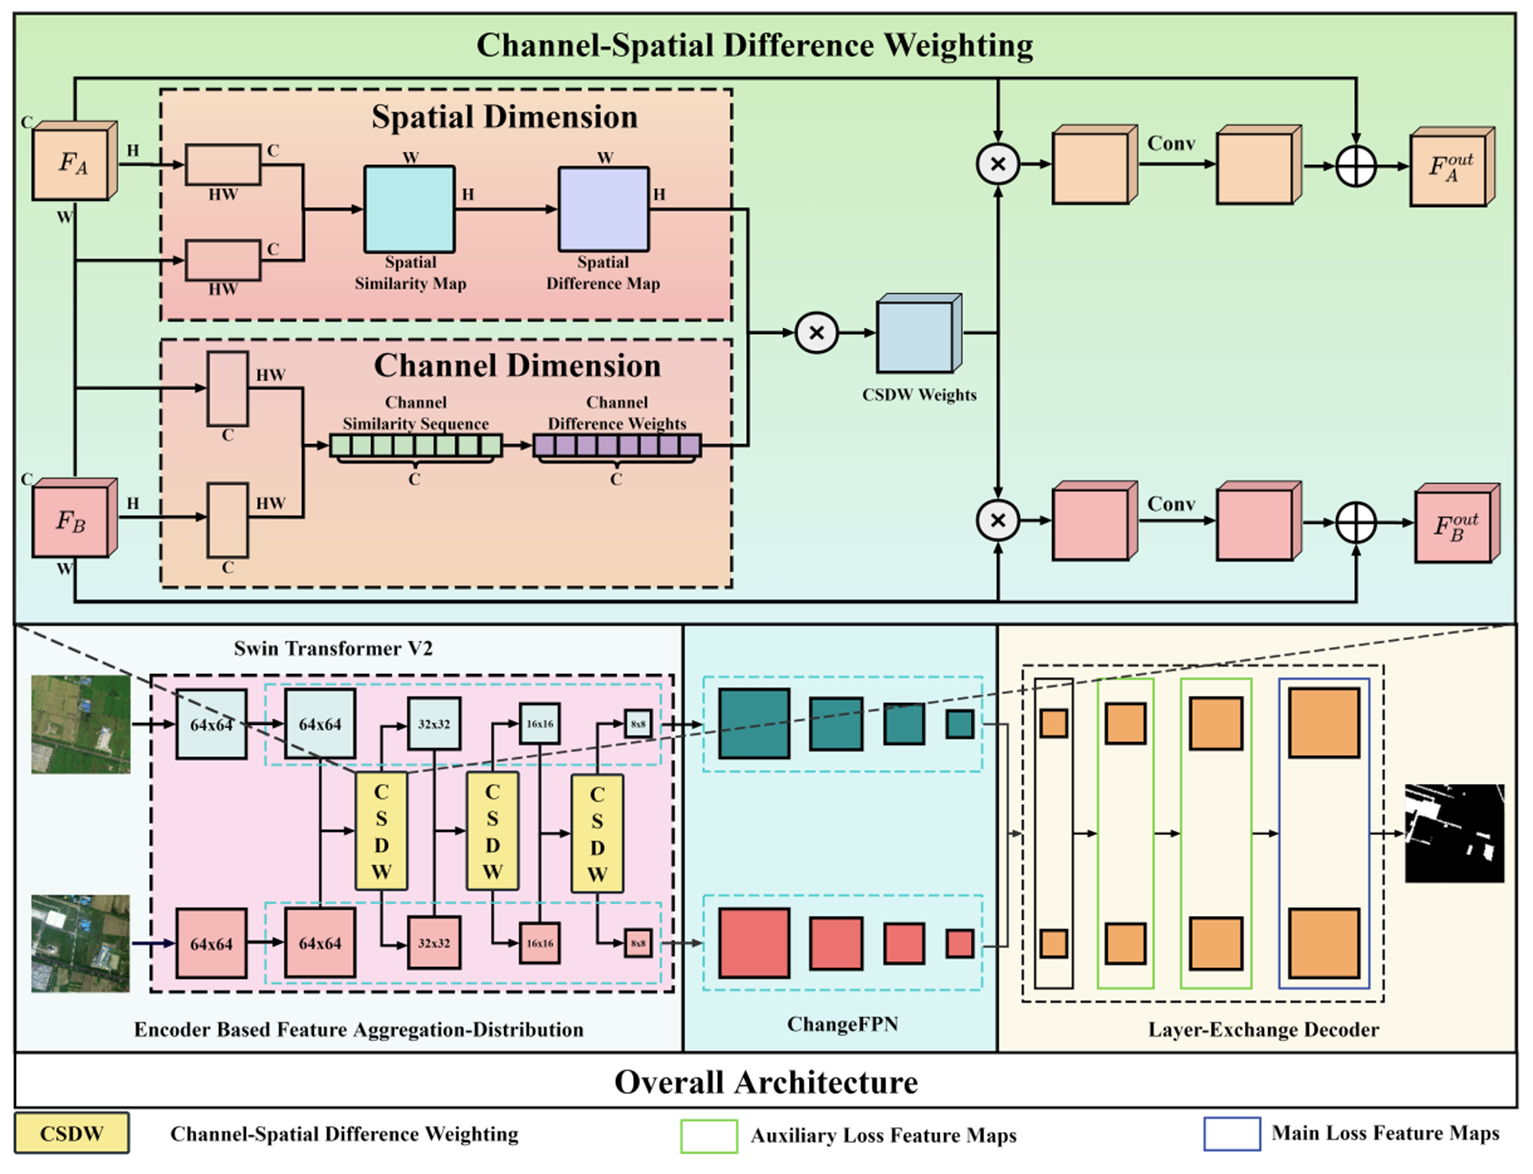
\includegraphics[width=\textwidth]{paper_figures/基于双时相遥感影像特征交互的变化检测算法研究/LENet/lenet.png}
  \caption{LENet 总体结构图}
  \label{fig:lenet}
\end{figure}

\begin{figure}[!htbp]
  \centering
  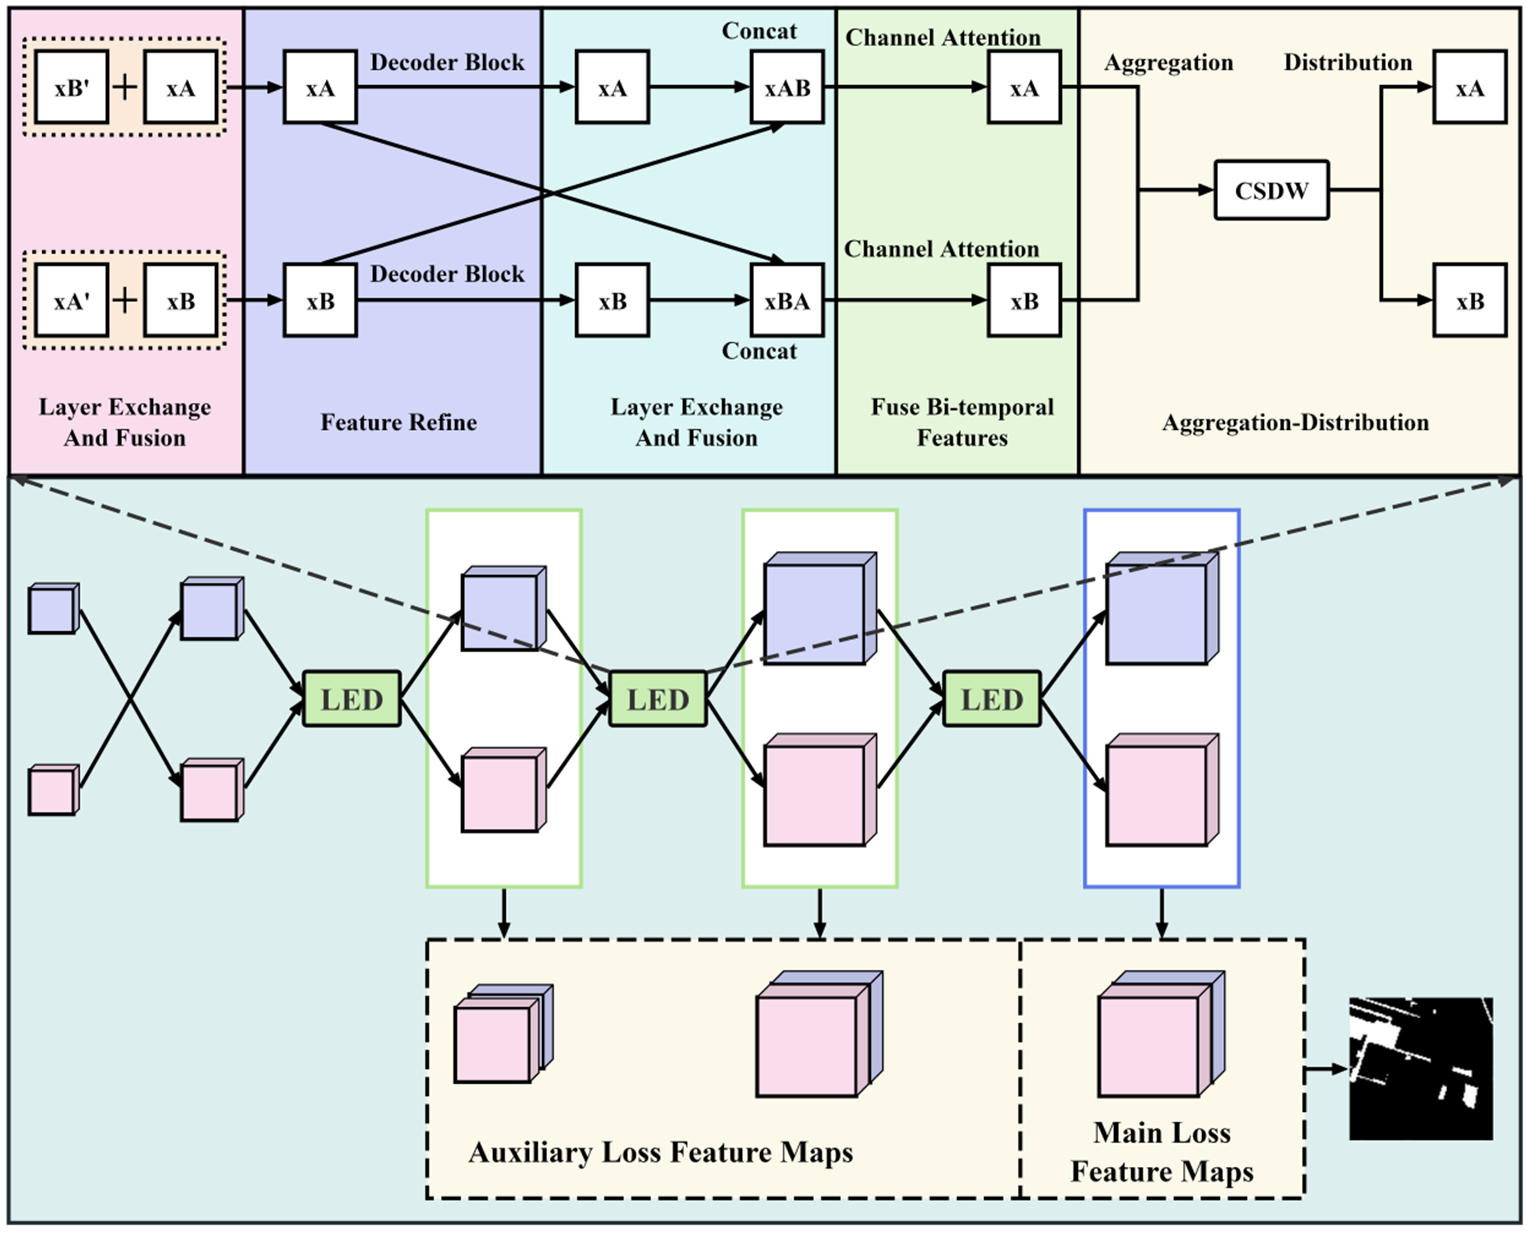
\includegraphics[width=\textwidth]{paper_figures/基于双时相遥感影像特征交互的变化检测算法研究/LENet/led.png}
  \caption{逐层交换解码器(LED)在 LENet 中的应用}
  \label{fig:led}
\end{figure}

\subsection{总体结构设计}
本章从两个角度对变化检测任务进行了优化。首先,在变化检测任务中,特征交互方法的优化可以增强模型感知差异特征的能力。为了实现这一点,设计了一个结合通道和空间维度计算差异特征的模块,即通道-空间差异加权(CSDW)模块。此外,在解码阶段,构建了一个基于层交换(Layer-Exchange,LE)方法的解码结构,以增强双时相特征的交互。通过在编码和解码阶段加强双时相特征的交互,本章的方法显著提高了变化检测模型的性能。如图~\ref{fig:lenet}所示,本章方法的结构如下:

骨干网络:采用Swin Transformer V2(SwinTV2)~\cite{liu_swin_2021-5}作为骨干网络,以利用其强大的全局信息学习能力。SwinTV2非常适合捕捉长距离依赖和层次特征,是变化检测任务的理想选择。

通道-空间差异加权(CSDW)模块:为了构建有效的双时相特征交互机制,提出了CSDW模块。该模块通过计算通道和空间维度上的差异,增强了模型对差异特征的敏感度。CSDW模块被集成到编码阶段,确保模型能够有效捕捉和表示双时相影像之间的变化。

ChangeFPN和层交换机制:采用ChangeFPN架构~\cite{dong_efficientcd_2024}来处理双时相特征金字塔。在这一阶段,双时相特征金字塔通过层交换机制进一步交互,增强了模型捕捉时间依赖性和空间相关性的能力。

逐层解码器(LED):在解码阶段,设计了一个简单而有效的特征融合模块,基于层交换机制,命名为逐层解码器(LED)。LED处理双时相特征金字塔,并生成最终的预测输出。

损失函数:在图~\ref{fig:lenet}的“整体架构”右侧,绿色框突出显示的特征图被拼接以计算辅助损失,权重为0.3。蓝色框突出显示的特征图被拼接以计算主损失,并作为推理输出。所采用的所有损失函数均为交叉熵损失。

通过集成这些组件,LENet在变化检测任务中实现了最先进的性能,展示了CSDW模块和层交换机制的有效性。

\subsection{基于通道-空间多维度的差异特征构建方式}
在变化检测模型中,孪生神经网络通常用于编码双时相影像,从而生成孪生特征金字塔。在编码过程中,对从SwinTV2的各个层次提取的双时相特征进行聚合和分布操作。采用这种方法,模型在孪生编码过程中基于双时相特征计算差异权重,并对编码阶段的双时相特征进行逐层加权。这增强了变化检测模型对变化特征的敏感性,使其能够更好地捕捉细微且复杂的变化。

\begin{figure}[!htbp]
  \centering
  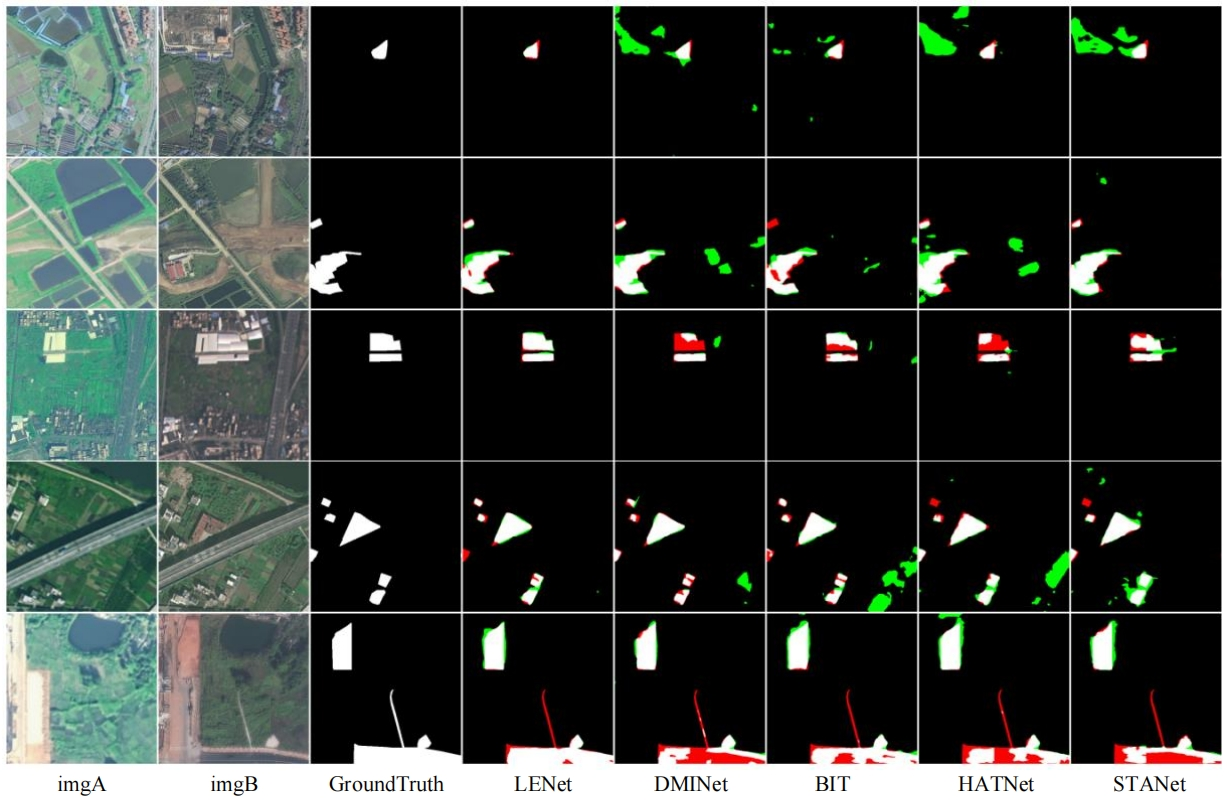
\includegraphics[width=\textwidth]{paper_figures/基于双时相遥感影像特征交互的变化检测算法研究/LENet/lenet_clcd.png}
  \caption{LENet 模型与对比模型在 CLCD 数据集上的可视化对比结果}
  \label{fig:lenet_clcd}
\end{figure}

在计算机视觉任务中,特征提取通常应用于图像数据,构建高维特征图矩阵。通道维度的特征主要通过对输入特征图应用多个卷积核的加权计算生成。由于卷积核初始化时具有不同的参数,每个通道中的特征自然集中于输入的不同方面,可能表示边缘、纹理、形状或更抽象的模式。另一方面,空间特征强调图像中像素或区域之间的关系和布局。空间特征反映了物体的结构特征,有助于识别和分析其形状、大小和布局。因此,特征图不仅在空间维度上对原始图像具有强大的表示能力,而且在通道维度上也具有丰富的信息表示能力。这种双重表示能力使得特征图在捕捉双时相图像中的局部和全局变化方面非常有效。

在本研究中,提出了通道-空间差异加权(CSDW)模块,用于学习双时相特征图在空间和通道维度上的差异,如上图~\ref{fig:lenet}所示。CSDW模块利用余弦相似度来计算差异特征,并对双时相特征图在空间和通道维度上应用差异权重。这种加权方法增强了双时相特征图对变化特征的敏感性,使得模型能够更有效地检测和表示变化。通过整合空间和通道差异信息,CSDW模块提供了一种全面的机制,用于捕捉局部和全局变化,从而提高了变化检测模型的整体性能。

CSDW模块通过计算两幅图像特征图之间的余弦相似度来生成变化权重,并将这些权重应用于特征图,从而实现特征差异的加权处理。CSDW模块的计算方法如下:
\begin{align}
F_c^{(i)} &= \mathcal{R}\bigl(\mathrm{permute}(F_i,(0,2,3,1)),\,(-1,C)\bigr), \quad i\in\{A,B\} \label{eq:lenet-1}\\
\phi_c &= \mathcal{R}\!\Bigl(\frac{F_c^{(A)}\cdot F_c^{(B)}}{\|F_c^{(A)}\|\;\|\;F_c^{(B)}\|},\,(N,H,W)\Bigr) \label{eq:lenet-2}\\
W_c &= 1 - \sigma\bigl(\mathrm{unsqueeze}(\phi_c,1)\bigr) \label{eq:lenet-3}\\
F_s^{(i)} &= \mathcal{R}(F_i,\,(N,C,-1)), \quad i\in\{A,B\} \label{eq:lenet-4}\\
\phi_s &= \mathcal{R}\!\Bigl(\frac{F_s^{(A)}\cdot F_s^{(B)}}{\|F_s^{(A)}\|\;\|\;F_s^{(B)}\|},\,(N,C)\Bigr) \label{eq:lenet-5}\\
W_s &= 1 - \sigma\bigl(\mathrm{unsqueeze}(\phi_s,1,1)\bigr) \label{eq:lenet-6}\\
W &= W_c \times W_s \label{eq:lenet-7}\\
F_i^{\mathrm{out}} &= \mathrm{Conv}_i\bigl(W \times F_i\bigr) + F_i,\quad i\in\{A,B\} \label{eq:lenet-8}
\end{align}

其中, \$F\_{A}\$ 和 \$F\_{B}\$ 表示维度为 \$(N, C, H, W)\$ 的输入特征图。
\(\mathcal{R}\) 表示用于改变输入维度的重塑函数,\(\Phi\) 表示余弦相似度结果(展平后特征图点积除以范数乘积),\(\sigma\) 表示 Sigmoid 函数,下标 \(c\) 和 \(s\) 分别表示通道和空间维度。
\texttt{Conv} 表示进一步处理输入特征图的卷积块。值得注意的是,选择通过乘法来融合 \$W\_{c}\$ 和 \$W\_{s}\$。从逻辑角度看,乘法类似于“与”操作:只有当通道和空间维度的变化权重 \$W\_{c}\$ 和 \$W\_{s}\$ 都较大时,最终权重 \$W\$ 才会显著提升。而加法则像“或”操作:只要有一个维度的权重较大,就能提升最终权重,可能放大伪变化信息。为了确保只有当空间差异权重和通道差异权重同时较高时总变化权重才上升,采用乘法融合它们。

最终输出特征图 \(F_{A}^{\mathrm{out}}\) 和 \(F_{B}^{\mathrm{out}}\) 是将残差模块的输出与原始输入特征图相加得到的。通过这一系列操作,模型能够高效地捕获并处理双时相图像的变化信息,增强对变化区域的敏感性和理解能力。

此外,在编码阶段提取的双时相特征金字塔上采用了ChangeFPN~\cite{dong_efficientcd_2024}。 该方法确保 Siamese 编码器不仅关注单幅时相图像的特征,还综合利用两幅图像的多尺度特征,从而增强特征表达的鲁棒性。通过整合多尺度特征并利用层交换机制,ChangeFPN 能够更好地捕获时序依赖和空间关联,进而实现更精确、更可靠的变化检测。

\subsection{结合特征层交换的变化检测解码器设计方法}
在变化检测任务中,解码阶段的目标是基于编码阶段提取的特征信息生成高质量的变化检测图。由于遥感影像中物体的尺度变化显著,通常在编码阶段构建特征金字塔,以增强模型对不同尺度目标的表示能力。因此,在解码阶段,模型可以利用在编码阶段提取的多尺度特征信息,提升变化检测的准确性和鲁棒性。

此外,双时相影像来自相同的地理位置,因此它们的特征之间具有很强的相关性。为了在变化检测模型中建立这些相关性,在逐层解码过程中引入了层交换特征融合机制,以促进双时相特征之间相关性的学习。在渐进解码阶段,使用了SwinTV2Block模块来优化特征,增强模型的拟合能力和捕捉复杂变化的能力。如图~\ref{fig:led}所示,详细解释了LENet中的层交换解码器(LED)。LED的结构如图~\ref{fig:led}上部所示。在此,$x_A'$ 和 $x_B'$ 分别表示来自上一层的双时相特征。首先,通过层交换机制,将来自两个时间影像的特征图 $x_A$ 和 $x_B$ 进行交叉融合,生成新的特征图 $x_A$ 和 $x_B$。这一交叉融合过程增强了双时相特征之间的相互作用,使模型能够更好地捕捉时间依赖性和空间相关性。 其次,这些特征图通过 SwinTV2 解码块(SwinTV2 Block)进一步优化,以增强特征表示能力。SwinTV2 块利用其层次化的注意力机制来捕捉局部和全局特征,从而提高模型在不同尺度上检测变化的能力。  

\begin{figure}[!htbp]
  \centering
  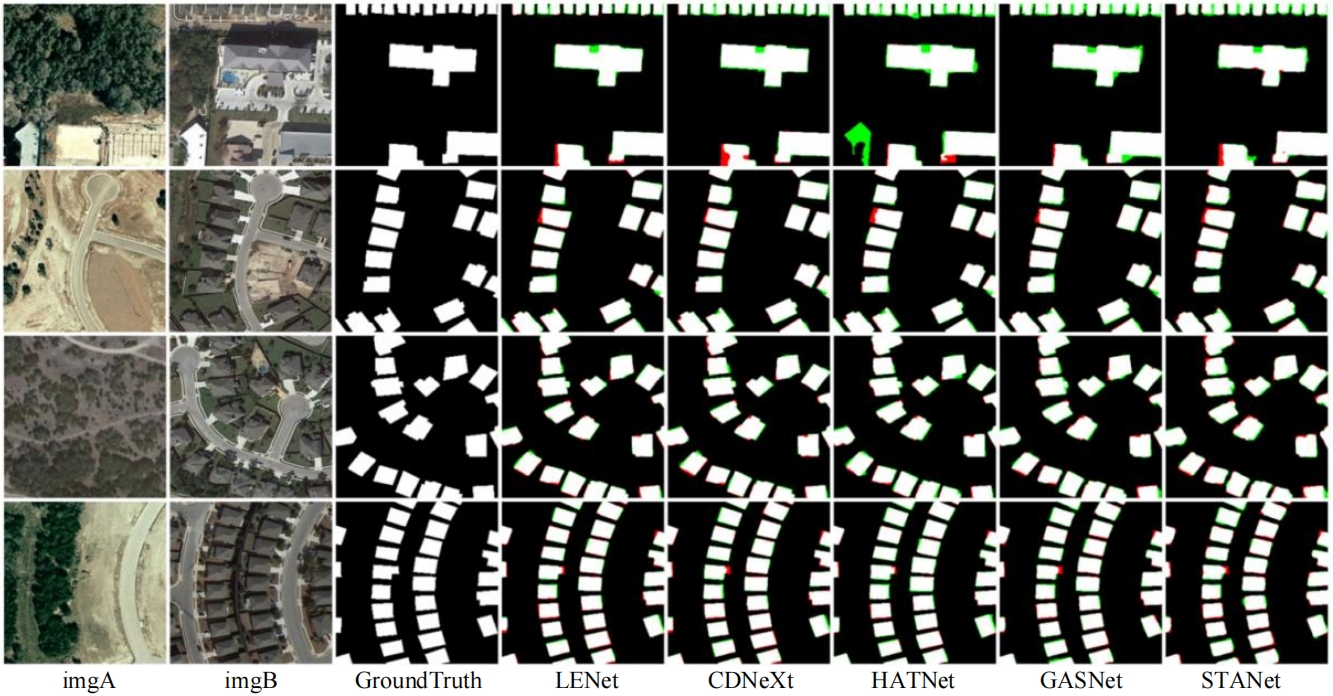
\includegraphics[width=\textwidth]{paper_figures/基于双时相遥感影像特征交互的变化检测算法研究/LENet/lenet_levir.png}
  \caption{LENet 模型与对比模型在 LEVIR-CD 数据集上的可视化对比结果}
  \label{fig:lenet_levir}
\end{figure}

此外,为了进一步促进特征的交互,基于层交换机制执行了残差特征融合。这种方法确保模型在融合交叉特征的同时,保留了原始特征中的重要信息。随后,特征图通过通道注意力机制加权,以强调重要特征。通道注意力机制根据每个通道与变化检测任务的相关性动态调整权重,从而增强模型对关键特征的敏感性。最后,通过基于CSDW的特征聚合-分布步骤进一步加权特征,以增强特征交互。处理后的特征图然后被拼接并输入到解码头中,生成变化检测结果。

其中,绿色框内拼接的特征图用于计算辅助损失,而蓝色框内拼接的特征图用于计算主损失,并作为预测结果的输出。在整个层交换解码器过程中,采用了多层次特征融合和交换机制,逐步优化和增强双时相影像的特征,从而提高变化检测的准确性和鲁棒性。

\begin{table}[!htbp]
  \centering
  \caption{LENet 模型与经典变化检测模型在 CLCD 数据集上的量化对比结果}
  \label{tab:lenet_clcd}
  \begin{tabular}{lcccc}
    \toprule
    Model                &  IoU   &   F1   &  Rec   &  Prec  \\
    \midrule
    ACABFNet~\cite{Song2023AxialCA}    & 51.45  & 67.94  & 63.63  & 72.88  \\
    STANet~\cite{chen_spatial-temporal_2020}      & 51.49  & 67.97  & 64.16  & 72.26  \\
    P2V~\cite{lin_transition_2023}        & 54.10  & 70.22  & 65.93  & 75.11  \\
    MSCANet~\cite{m_liu_cnn-transformer_2022}     & 55.83  & 71.65  & 67.07  & 76.91  \\
    HATNet~\cite{Xu2024HybridAT}    & 56.90  & 72.53  & 69.42  & 75.94  \\
    BIT~\cite{chen_remote_2022}         & 58.36  & 73.71  & 66.63  & 82.47  \\
    DSIFN~\cite{Zhang2020ADS}       & 59.42  & 74.54  & 67.86  & 82.69  \\
    MIN-Net~\cite{Zhou2024MultistageIN}     & 62.08  & 76.60  & 75.70  & 77.53  \\
    AMTNet~\cite{Liu2023AnAM}      & 62.35  & 76.81  & 75.06  & 78.64  \\
    SAM-CD2~\cite{Sun2024SegmentAM}     & 62.54  & 76.95  & 71.60  & 83.17  \\
    CGNet~\cite{han_change_2023}       & 62.67  & 77.05  & 71.71  & 83.25  \\
    CACG-Net~\cite{Liu2024CandidateAwareAC}    & 64.76  & 78.61  & 76.71  & 80.61  \\
    EfficientCD~\cite{dong_efficientcd_2024}& 65.14  & 78.89  & 75.83  & 82.21  \\
    LENet                & \textbf{66.83} & \textbf{80.12} & \textbf{77.09} & \textbf{83.39} \\
    \bottomrule
  \end{tabular}
\end{table}

\begin{table}[!htbp]
  \centering
  \caption{不同模型与 LENet 模型在 LEVIR-CD 数据集上的量化对比结果}
  \label{tab:lenet_levir}
  \begin{tabular}{lcccc}
    \toprule
    Model                   &   IoU   &   F1   &   Rec   &  Prec   \\
    \midrule
    STANet~\cite{chen_spatial-temporal_2020}        &  81.85  &  90.02 &  87.13  &  93.10  \\
    ChangeFormer~\cite{bandara2022transformer}  &  82.66  &  90.50 &  90.18  &  90.83  \\
    Changer~\cite{Fang2022ChangerFI}       &   --    &  92.06 &  90.56  &  93.61  \\
    SSCD~\cite{Wang2024SummatorSubtractorNM}          &  82.78  &  90.58 &  89.08  &  92.12  \\
    CDMamba~\cite{zhang_cdmamba_2025}       &  83.07  &  90.75 &  90.08  &  91.43  \\
    DMATNet~\cite{Song2022RemoteSI}       &  84.13  &  90.75 &  89.98  &  91.56  \\
    GASNet~\cite{zhang_global-aware_2023}        &   --    &  91.21 &  90.62  &  91.82  \\
    Hybrid-MambaCD~\cite{Feng2025HybridMambaCDHM} &  84.31  &  91.48 &  90.78  &  92.20  \\
    ACAHNet~\cite{Zhang2023AsymmetricCH}       &  84.35  &  91.51 &  90.68  &  92.36  \\
    HATNet~\cite{Xu2024HybridAT}        &  84.41  &  91.55 &  90.23  &  92.90  \\
    ConMamba~\cite{Dong2024ConMambaCA}      &   --    &  91.70 &  90.06  &  93.14  \\
    FEMCD~\cite{Xing2025FrequencyEnhancedMF}         &   --    &  92.02 &  90.88  &  93.18  \\
    IMDCD~\cite{Liu2024IterativeMD}         &  84.66  &  91.34 &  91.12  &  91.56  \\
    DED-SAM~\cite{Qiu2025DEDSAMAdaptingSA}       &  85.11  &  92.00 &  90.47  &  93.51  \\
    PCAANet~\cite{Xu2023ProgressiveCA}       &  85.22  &  92.02 &  90.67  &  93.41  \\
    MSA~\cite{Huang2025MSAMS}           &  85.34  &  92.09 &  90.55  &  93.68  \\
    HFIFNet~\cite{Han2025HFIFNetHF}       &  85.46  &  92.16 &  90.09  &  93.37  \\
    EfficientCD~\cite{dong_efficientcd_2024}   &  85.55  &  92.21 &  91.22  &  93.23  \\
    SAM-CD2~\cite{Sun2024SegmentAM}       &  85.59  &  92.24 &  90.93  &  93.58  \\
    CACG-Net~\cite{Liu2024CandidateAwareAC}      &  85.68  &  92.29 &  92.41  &  92.16  \\
    CDNeXt~\cite{wei_robust_2024}        &  85.86  &  92.39 &  90.92  &  93.91  \\
    RSBuilding~\cite{wang_rsbuilding_2024}    &  86.19  &  92.59 &  91.80  &  93.39  \\
    LENet                   & \textbf{86.30} & \textbf{92.64} &  91.22  & \textbf{94.12} \\
    \bottomrule
  \end{tabular}
\end{table}



\subsection{实验结果与分析}

\begin{figure}[!htbp]
  \centering
  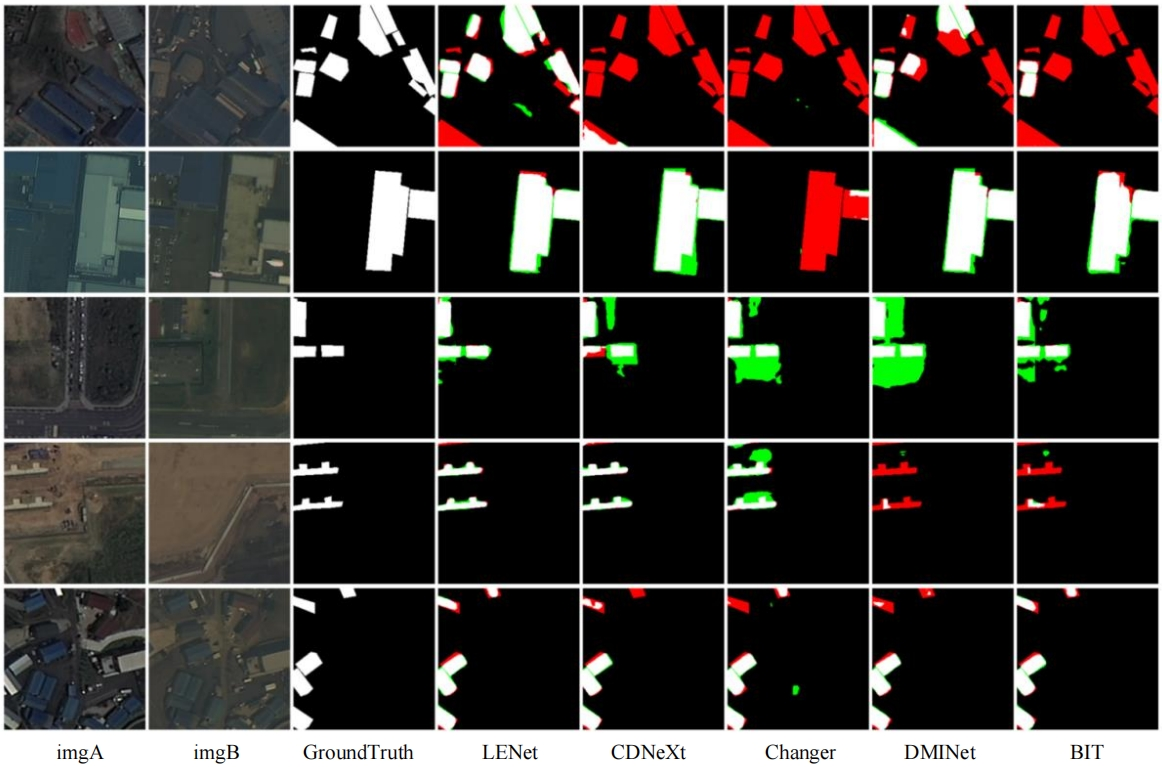
\includegraphics[width=\textwidth]{paper_figures/基于双时相遥感影像特征交互的变化检测算法研究/LENet/lenet_s2looking.png}
  \caption{LENet 模型与对比模型在 S2Looking 数据集上的可视化对比结果}
  \label{fig:lenet_s2looking}
\end{figure}


\begin{table}[!htbp]
  \centering
  \caption{不同模型与 LENet 模型在 S2Looking 数据集上的量化对比结果}
  \label{tab:lenet_s2looking}
  \begin{tabular}{lcccc}
    \toprule
    Model              &  IoU   &   F1   &   Rec   &  Prec  \\
    \midrule
    BIT~\cite{chen_remote_2022}       & 47.94  & 64.81  & 58.15   & 73.20  \\
    HATNet~\cite{Xu2024HybridAT}    & 47.08  & 64.02  & 60.90   & 67.48  \\
    FHD~\cite{pei_feature_2022}       & 47.33  & 64.25  & 56.71   & 74.09  \\
    CGNet~\cite{han_change_2023}     & 47.41  & 64.33  & 59.38   & 70.18  \\
    DMINet~\cite{feng_change_2023}    & 48.33  & 65.16  & 62.13   & 68.51  \\
    PCAANet~\cite{Xu2023ProgressiveCA}   & 48.54  & 65.36  & 61.54   & 69.68  \\
    HFIFNet~\cite{Han2025HFIFNetHF}   & 48.54  & 65.35  & 61.04   & 70.33  \\
    CDNeXt~\cite{wei_robust_2024}    & 50.05  & 66.71  & 63.08   & 70.78  \\
    Changer~\cite{Fang2022ChangerFI}   & 50.47  & 67.08  & 62.04   & 73.01  \\
    LENet              & \textbf{51.19} & \textbf{67.71} & 61.90 & \textbf{74.72} \\
    \bottomrule
  \end{tabular}
\end{table}


\begin{table}[!htbp]
  \centering
  \caption{不同模型与 LENet 模型在 PX-CLCD 数据集上的量化对比结果}
  \label{tab:lenet_pxclcd}
  \begin{tabular}{lcccc}
    \toprule
    Model              &  IoU   &   F1   &   Rec   &  Prec  \\
    \midrule
    HATNet~\cite{Xu2024HybridAT}    & 88.99  & 94.18  & 93.83   & 94.53  \\
    MSCANet~\cite{m_liu_cnn-transformer_2022}   & 89.00  & 94.18  & 93.95   & 94.41  \\
    BIT~\cite{chen_remote_2022}      & 90.78  & 95.17  & 94.80   & 95.54  \\
    GASNet~\cite{zhang_global-aware_2023}    & 92.51  & 96.11  & 96.42   & 95.80  \\
    DMINet~\cite{feng_change_2023}    & 92.83  & 96.28  & 96.31   & 96.25  \\
    SNUNet3+~\cite{miao_snunet3_2024}  & 93.61  & 96.64  & 96.79   & 96.60  \\
    CGNet~\cite{han_change_2023}     & 93.82  & 96.81  & 97.33   & 96.30  \\
    LENet               & \textbf{94.86} & \textbf{97.36} & \textbf{97.08} & \textbf{97.65} \\
    \bottomrule
  \end{tabular}
\end{table}


\subsubsection{实验结果量化指标与可视化分析}
在CLCD、LEVIR-CD、S2Looking 以及 PX-CLCD 数据集上,将 LENet与多种最先进算法进行了 详细的对比实验。正如表~\ref{tab:lenet_clcd}、表~\ref{tab:lenet_levir}、表~\ref{tab:lenet_s2looking}和表~\ref{tab:lenet_pxclcd}所示,LENet 在所有主要评价指标上均优于相关对比模型,表现出卓越的变化检测能力。

\begin{figure}[!htbp]
  \centering
  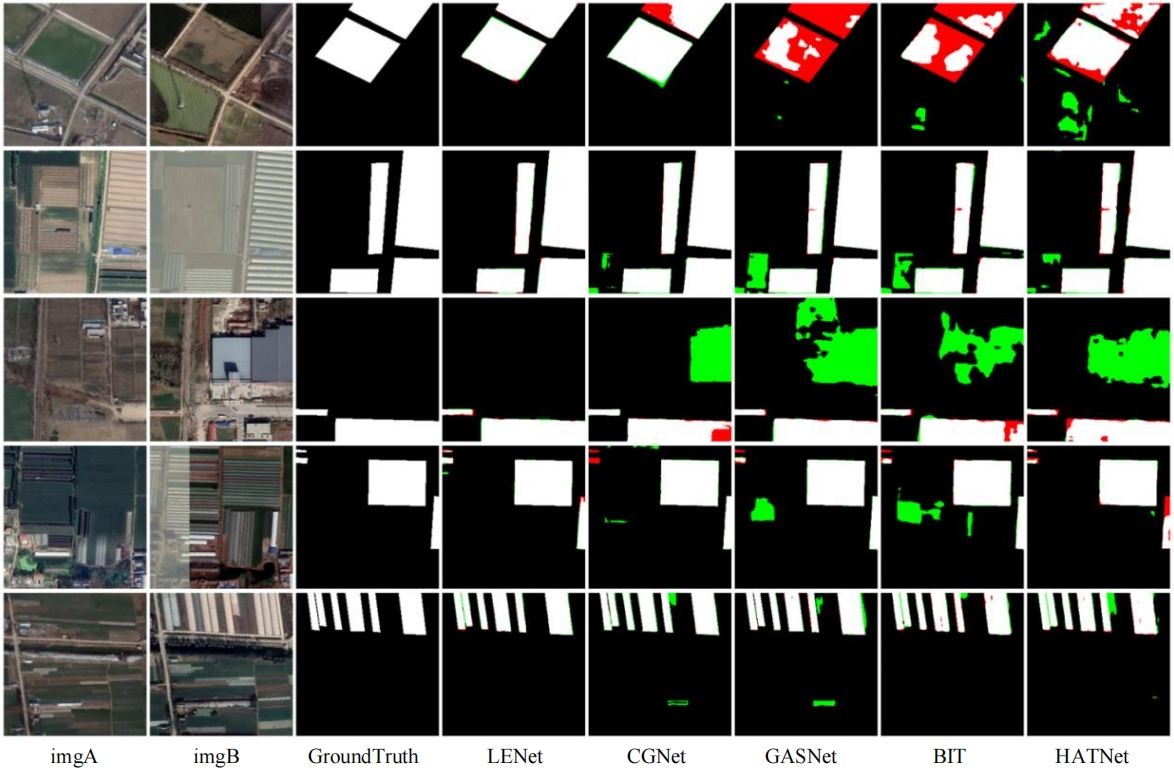
\includegraphics[width=\textwidth]{paper_figures/基于双时相遥感影像特征交互的变化检测算法研究/LENet/lenet_pxclcd.png}
  \caption{LENet 模型与对比模型在 PX-CLCD 数据集上的可视化对比结果}
  \label{fig:lenet_pxclcd}
\end{figure}

选取了近年来在差异特征计算~\cite{feng_change_2023}、与 AI 基础模型融合~\cite{Sun2024SegmentAM, Qiu2025DEDSAMAdaptingSA}、大规模数据集利用~\cite{wang_rsbuilding_2024}、注意力机制~\cite{Song2023AxialCA, chen_remote_2022} 等领域取得进展的代表模型作为对比,以充分展示 LENet 的优势。为保证实验公平,对于原文未给出结果的模型,均进行了重训练。考虑到二分类变化检测任务的特点,将前景变化类别的 IoU 作为主要评价指标,同时结合 F1、Recall 和 Precision 对模型整体性能进行全面评估。

在 CLCD、LEVIR‐CD、PX‐CLCD 和 S2Looking 数据集上的实验结果表明,LENet 在多项关键指标上均取得了优异成绩。以 CLCD 和 LEVIR‐CD 数据集为例,LENet 分别在 IoU、F1、Recall、Precision 上显著超越最优对手 EfficientCD(IoU 从 65.14\% 提升至 66.83\%)与 RSBuilding(IoU 从 86.19\% 提升至 86.30\%),展现了对微小农田变化和大规模建筑物变化的高灵敏度与鲁棒性。

在更具挑战性的 PX‐CLCD 和 S2Looking 上,LENet 同样表现出色:PX‐CLCD IoU 达到 94.86\%,超越 CGNet(93.82\%)与 SNUNet3+(93.61\%);S2Looking 上 IoU/F1 达到 51.19\%/67.71\%,较最佳方法 Changer 分别提升 0.72 和 0.63 个百分点,Precision 提升尤为显著(74.72\% vs. 73.01\%)。此外,图~\ref{fig:lenet_clcd}、图~\ref{fig:lenet_levir}、图~\ref{fig:lenet_s2looking}和图~\ref{fig:lenet_pxclcd}展示了 LENet 在四个数据集上的可视化结果(TP: 白色,TN: 黑色,FP: 绿色,FN: 红色),结果表明 LENet 在微小区域变化捕捉与噪声抑制方面均有突出表现。图~\ref{fig:lenet_rader}则以雷达图形式直观展现各方法在不同数据集和指标上的综合表现,LENet 的“蜘蛛网”面积最为宏大,进一步验证了其通用性与稳定性。

\subsubsection{消融研究}
\paragraph{消融研究}
针对 CLCD、LEVIR-CD、PX-CLCD 和 S2Looking 四个数据集的 IoU 指标进行的消融研究揭示了在编码阶段引入 CSDW 模块和在解码阶段加入 LED 对 LENet 性能的显著提升。如表\ref{tab:lenet_ablation}所示,“Encoder (CSDW)” 表示在编码阶段使用 CSDW 模块作为聚合-分布模块;“Decoder (LED)” 表示在解码阶段使用基于层交换的解码器 (LED)。基线条件下,使用基于 SwinTV2 的常规模型编码器和逐层上采样的常规模型解码器,所有数据集的性能均较低:LEVIR-CD 数据集 IoU 为 84.85,PX-CLCD 为 93.74,CLCD 为 59.96,S2Looking 为 49.12。

\paragraph{编码器 (CSDW) 的效果}
在编码阶段加入 CSDW 模块后,IoU 分数显著提升。例如,LEVIR-CD 数据集从 84.85 提升至 85.53,PX-CLCD 从 93.74 提升至 94.34;CLCD 从 59.96 提升至 61.03,S2Looking 从 49.12 提升至 50.05。这表明 CSDW 模块能够增强模型在编码阶段捕捉和表示差异特征的能力。

\paragraph{解码器 (LED) 的效果}
仅在解码阶段引入 LED 而不使用 CSDW 时,各数据集的 IoU 同样有所提升:LEVIR-CD 提升至 86.08,PX-CLCD 提升至 94.40,CLCD 提升至 61.74,S2Looking 提升至 50.76。这突出表明 LED 在解码阶段通过增强特征交互与融合,能更好地利用时序依赖和空间相关性。

\paragraph{联合使用 CSDW 与 LED}
当同时集成编码器 (CSDW) 与解码器 (LED) 时,IoU 得分进一步提升,展示了二者的互补作用:LEVIR-CD 达到 86.30,PX-CLCD 达到 94.86,CLCD 提升至 66.83,S2Looking 达到 51.19。这表明将 CSDW 与 LED 相结合可在双时相特征的表示与融合上获得最全面的提升。


\paragraph{基于空间差异与通道差异的消融(表~\ref{tab:lenet_ablation_csdw})}
在 CSDW 模块中分别禁用或启用了空间差异与通道差异,并在表~\ref{tab:lenet_ablation_csdw}中展示了结果:  
\begin{itemize}
  \item 当空间差异与通道差异均关闭时,模型在 LEVIR-CD、PX-CLCD、CLCD、S2Looking 上的 IoU 分别为 86.08\%, 94.40\%, 61.74\%, 50.76\%。
  \item 仅启用空间差异时,IoU 分别提升至 86.12\%, 94.53\%, 63.35\%, 50.94\%。
  \item 仅启用通道差异时,IoU 分别提升至 86.20\%, 94.65\%, 64.12\%, 50.88\%。
  \item 同时启用空间差异与通道差异时,IoU 分别达到 86.30\%, 94.86\%, 66.83\%, 51.19\%。
\end{itemize}
该结果进一步验证了 CSDW 模块中空间差异与通道差异的显著互补性和协同增益。


\begin{figure}[!htbp]
  \centering
  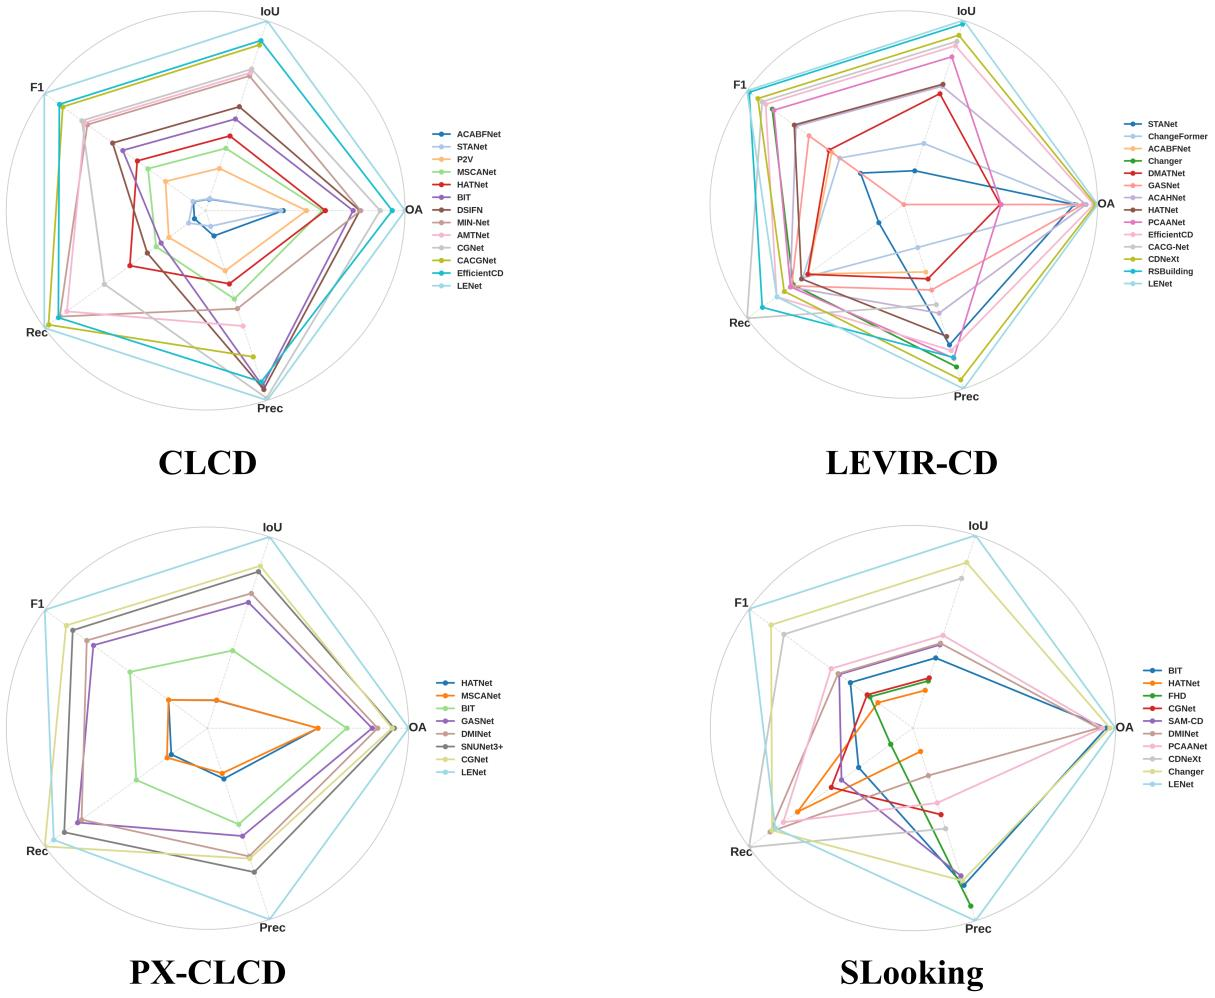
\includegraphics[width=\textwidth]{paper_figures/基于双时相遥感影像特征交互的变化检测算法研究/LENet/lenet_rader.png}
  \caption{LENet模型与其他模型在多个数据集上的对比雷达图。}
  \label{fig:lenet_rader}
\end{figure}



\begin{table}[!htbp]
  \centering
  \caption{基于IoU指标的LENet模型消融实验}
  \label{tab:lenet_ablation}
  \begin{tabular}{lcccccc}
    \toprule
    Model & \makecell{Encoder\\(CSDW)} & \makecell{Decoder\\(LED)} & LEVIR-CD & PX-CLCD & CLCD  & S2Looking \\
    \midrule
    LENet               & $\times$      & $\times$      & 84.85    & 93.74   & 59.96 & 49.12     \\
                        & $\checkmark$  & $\times$      & 85.53    & 94.34   & 61.03 & 50.05     \\
                        & $\times$      & $\checkmark$  & 86.08    & 94.40   & 61.74 & 50.76     \\
                        & $\checkmark$  & $\checkmark$  & 86.30    & 94.86   & 66.83 & 51.19     \\
    \bottomrule
  \end{tabular}
\end{table}


% \begin{table}[!htbp]
%   \centering
%   \caption{基于IoU指标的CSDW模块消融实验}
%   \label{tab:5-6}
%   \begin{tabular}{lcccccc}
%     \toprule
%     Module & Spatial Difference & Channel Difference & LEVIR-CD & PX-CLCD & CLCD  & S2Looking \\
%     \midrule
%     CSDW               & $\times$      & $\times$      & 86.08    & 94.40   & 61.74 & 50.76     \\
%                        & $\checkmark$  & $\times$      & 86.12    & 94.53   & 63.35 & 50.94     \\
%                        & $\times$      & $\checkmark$  & 86.20    & 94.65   & 64.12 & 50.88     \\
%                        & $\checkmark$  & $\checkmark$  & 86.30    & 94.86   & 66.83 & 51.19     \\
%     \bottomrule
%   \end{tabular}
% \end{table}

\begin{table}[!htbp]
  \centering
  \caption{基于IoU指标的CSDW模块消融实验}
  \label{tab:lenet_ablation_csdw}
  \begin{tabular}{lcccccc}
    \toprule
    Module 
      & \makecell{Spatial\\Difference} 
      & \makecell{Channel\\Difference} 
      & LEVIR-CD 
      & PX-CLCD 
      & CLCD  
      & S2Looking \\
    \midrule
    CSDW               & $\times$      & $\times$      & 86.08    & 94.40   & 61.74 & 50.76     \\
                       & $\checkmark$  & $\times$      & 86.12    & 94.53   & 63.35 & 50.94     \\
                       & $\times$      & $\checkmark$  & 86.20    & 94.65   & 64.12 & 50.88     \\
                       & $\checkmark$  & $\checkmark$  & 86.30    & 94.86   & 66.83 & 51.19     \\
    \bottomrule
  \end{tabular}
\end{table}



\subsection{讨论}

\subsubsection{变化检测中的特征交互}
在变化检测任务中,特征交互是提升模型性能的关键因素。特征交互能够在双时相图像之间进行充分的信息交换,从而增强模型对双时相数据的表示能力。通过特征交互机制,模型对差异区域的敏感性得以提升,促进双时相特征的融合与信息共享。此外,层交换机制仅在适当的位置交换双时相图像的特征,而不改变模型结构,从而在不增加计算负担的前提下实现了双时相特征的交互。

具体地,通道-空间差异加权(CSDW)模块在编码阶段对双时相特征应用加权处理,使双时相特征的关注区域更加聚焦于变化区域,从而构建了多层次的特征交互。在解码阶段,采用层交换机制实现双时相特征的交叉融合,随后在解码过程中再次通过 CSDW 进行特征加权,进一步优化变化区域的特征表示。该双重策略保证了模型既能有效捕捉局部变化,也能获取全局变化信息,进而实现更准确、更鲁棒的变化检测结果。

\subsubsection{变化检测中的层交换机制}
在变化检测任务中,层交换机制为双时相特征交互提供了一种创新的解决方案。由于双时相图像来源于同一地理位置,其特征具有很高的相关性。通过在解码阶段采用层交换机制,实现了双时相特征的跨时序交互,增强了变化特征的表达能力。

与传统的特征融合方法相比,层交换机制直接交换双时相特征层,既能在深层次实现信息融合,又能保持模型结构的简洁性和计算效率。通过对应特征层的交换,层交换机制使模型在不增加参数量的情况下高效地整合双时相信息,强化了双时相特征之间的信息交换,从而提升了变化检测模型的表达能力。

本章的实验结果表明,该层交换解码设计显著提升了模型在变化检测任务中的性能,在准确性和鲁棒性方面均取得了优异表现。层交换机制不仅增强了模型捕捉时序依赖和空间相关性的能力,还确保了计算效率,是遥感变化检测任务中实用且高效的解决方案。

\subsubsection{变化检测中的通道–空间差异}
在 LENet 中,本章从两个互补的角度对变化特异性差异进行建模:空间差异与通道差异。空间差异在空间平面上计算余弦相似度,对边缘和轮廓等局部变化尤为敏感;通道差异在特征图通道维度上计算余弦相似度,捕捉双时相特征图之间的整体语义变化。为了确保只有在空间差异和通道差异同时显著时才增强变化响应,CSDW 模块采用乘法而非加法融合这两种差异(加法类似“或”操作,可能放大伪变化信息)。融合后的权重图既能放大细粒度的局部变化,也能反映全局的通道级语义变化。

消融研究(表~\ref{tab:lenet_ablation_csdw})显示:仅启用空间差异或仅启用通道差异时,LEVIR-CD、PX-CLCD、CLCD 和 S2Looking 上的 IoU 均有所提升;但只有在同时启用空间差异与通道差异时,IoU 分别达到最高的 86.30\%、94.86\%、66.83\% 和 51.19\%。这证实了空间信息与通道信息并非冗余,而是真正互补:空间加权确保对局部变化区域的高灵敏度,通道加权则提供了对全局变化特征的语义理解。


\subsection{小结}

本研究从空间维度和通道维度同时计算双时相影像的变化信息,提出了通道-空间差异加权(CSDW)模块,以优化双时相特征间差异特征的学习;此外,还在解码阶段设计了基于层交换机制的解码模块(LED),以增强双时相特征在解码过程中的交互能力。在 CLCD、LEVIR-CD、PX-CLCD 和 S2Looking 四个数据集上的大规模实验,验证了 LENet 在多种评价指标上的优越性能。未来工作中,将继续探索在变化检测架构中仅依赖特征交换而非传统差异特征计算模块的可能性,并尝试将特征交换机制用于自监督学习,以减少对大规模标注数据的依赖。

